\documentclass[a4paper, fontsize = 7pt, landscape]{scrartcl}
\usepackage{layout_and_colours}



\author{Jil Zerndt}
\title{Analysis I Cheatsheet}
\subtitle{}


\createtitlepagestyle
\createmainpagestyle

\begin{document}
	\begin{multicols*}{3}
		\thispagestyle{TitlePageStyle}
		\maketitle
        \vspace{1mm}
		%Basics
            \section{Basics}
                
\graphicspath{ {./Images/} }
\begin{corollary}[]{Archimedisches Prinzip}
    Sei $x \in \R$ mit $x > 0$ und $y \in \R$. Dann gibt es $n \in \N$ mit $y \leq nx$
\end{corollary}
\begin{theorem}{Ungleichungen}
    $\forall x,y \in \R$
    \begin{equation*}
        \begin{array}{lclc}
            (i) & |x| \geq 0 & (iii) & |x+y| \leq |x| + |y|\\
            (ii) & |xy| = |x||y| & (iv) & |x+y| \geq ||x| - |y||
        \end{array}
    \end{equation*}
\end{theorem}
\begin{theorem}[]{Young'sche Ungleichung}
       $\forall \varepsilon > 0,~\forall y \in \R gilt:
       \hspace{1mm}
       2 |xy| \leq \varepsilon x^2 + \frac{1}{\varepsilon} y^2$
\end{theorem}
\begin{lemma}[]{Bernoulli Ungleichung}
    $(1 + x)^n \geq 1 + nx \quad \forall n \in \N, x > -1$
\end{lemma}
\begin{definition}{Kardinalität}
    \begin{itemize}
        \item Mengen $X$, $Y$ heissen \emph{gleichmächtig}, falls es eine \underline{Bijektion} $f: X \to Y$ gibt.
        \item Menge $X$ ist \emph{endlich}, falls entweder $X = \emptyset$ ($\card X = 0$) oder $\exists n \in \N$, sodass $X$ und $\{1,2,\ldots,n\}$ ($\card X = n$) gleichmächtig sind.
        \item Menge $X$ ist \emph{abzählbar}, falls sie endlich oder gleichmächtig wie $\N$ ist.
    \end{itemize}
\end{definition}
\begin{definition}{Beschränktheit}
    $A \subseteq \R$ eine Teilmenge.
    \begin{itemize}
        \item $c \in \R$ ist eine \emph{obere Schranke} von A falls $\forall a \in A: a\leq c$ ($A$ \textit{nach oben beschränkt}).
        \item $c \in \R$ ist eine \emph{untere Schranke} von A falls $\forall a \in A: a \geq c$ ($A$ \textit{nach unten beschränkt}).
        \item $A$ heisst \textit{beschränkt}, wenn nach oben und unten beschränkt.
        \item $m \in \R$ heisst \emph{Maximum} von $A$ falls $m \in A$ und $m$ obere Schranke.
        \item $m \in \R$ heisst \emph{Minimum} von $A$ falls $m \in A$ und $m$ untere Schranke.
    \end{itemize}
\end{definition}


\begin{definition}{Intervalle}
    Ein \emph{abgeschlossenes Intervall} ist eine Teilmenge $I \subseteq \R$ der Form
    \begin{itemize}
        \item Abgeschlossen:
            $[a, b]=\{x \in \mathbb{R} \mid a \leq x \leq b\}$
        \item Offen:
            $(a, b)=\{x \in \mathbb{R} \mid a<x<b\}$
        \item Halboffen:
            $[a, b)=\{x \in \mathbb{R} \mid a \leq x<b\}$
        \item Unendlich:
            $[a, \infty)=\{x \in \mathbb{R} \mid a \leq x\}$
    \end{itemize}
\end{definition}



                
\begin{KR}{Polynomdivision}\\
    $\frac{P(x)}{q(x)} = S(x) + \frac{r(x)}{q(x)}$ \qquad $P,q,S,r$ Polynome\\
\emph{!} Vorzeichen von Nullstellen umdrehen.
\tcblower
$$
\begin{array}{cc}
\left(x^3-2 x^2-5 x-6\right):(x-1)=x^2-x-6 & \mid x^3: x=x^2 \\
-\left(x^3-x^2\right) & \mid-x^2: x=-x \\
-x^2-5 x & \\
-\left(x^2-x\right) & \mid-6 x: x=-6 \\
\hline-(-6 x+6) &
\end{array}
$$

Eine Polynomfunktion vom Grad $n$ hat höchstens $n$ reelle Nullstellen.
$$
f(x)=a_n \cdot\left(x-x_1\right) \cdot\left(x-x_2\right) \cdot \ldots \cdot\left(x-x_n\right)
$$
\end{KR}



                \raggedcolumns
                \columnbreak
                \subsection{Trigonometrie}
                \subsubsection{Trigonometrische Funktionen}
\begin{iequation}[align*]
	\tikz[remember picture] \coordinate(sinanchor) at (0,0); \sin x &= \sum_{n=0}^{\infty} \frac{(-1)^n x^{2n + 1}}{(2n+1)!} = x - \frac{x^3}{3!} + \frac{x^5}{5!}\ldots ~ \text{stetig}\\
	\tikz[remember picture] \coordinate(cosanchor) at (0,0); \cos x &= \sum_{n=0}^{\infty} \frac{(-1)^n x^{2n}}{(2n)!} = 1 - \frac{x^2}{2!} + \frac{x^4}{4!}\ldots \hspace{3.8mm} \text{stetig}\\
	\tan x &= \frac{\sin x}{\cos x} \hspace{10mm} \cot x = \frac{\cos x}{\sin x} \tikz[remember picture] \coordinate(trigfunkanchor) at (0,0);
\end{iequation}
\begin{tikzpicture}[remember picture, overlay]
	\node[overlaynote, text width = 28mm, anchor = west] at ($(trigfunkanchor) + (0.5,0.25)$) {$\pi$: kleinste strikt positive Nullstelle von $\sin$.};
	\node[overlaynote, rotate = 90] at ($(trigfunkanchor) + (3,2)$) {$\cos(x) = \sin \left(x + \frac{\pi}{2}\right)$};
	\node[overlaynote, rotate = 20, above left = 3mm and 2mm of sinanchor] (sinnote) {ungerade};
	\draw[overlayarrow] (sinnote) to[bend right] (sinanchor);
	\node[overlaynote, rotate = 20, above left = 3mm and 2mm of cosanchor] (cosnote) {gerade};
	\draw[overlayarrow] (cosnote) to[bend right] (cosanchor);
\end{tikzpicture}
\begin{comment}
\begin{flushleft}
    \begin{tikzpicture}[remember picture]
        \begin{axis} [
            samples=200,
            axis x line = middle,
            axis y line = left,
            grid = both,
            xtick={-pi,3*-pi/4,-pi/2,-pi/4,0,pi/4,pi/2,3*pi/4,pi,5*pi/4,3*pi/2,7*pi/4,2*pi},
            ytick={-1, -0.5, 0, 0.5, 1},
            xticklabels={$-\pi$, $-\frac{3\pi}{4}$, $-\frac{\pi}{2}$, $-\frac{\pi}{4}$, $0$,$\frac{\pi}{4}$,$\frac{\pi}{2}$,$\frac{3\pi}{4}$,$\pi$,$\frac{5\pi}{4}$,$\frac{3\pi}{2}$,$\frac{7\pi}{4}$,$2\pi$},
            width = 0.8\linewidth,
            height = 40mm,
            xmin=0,
            ymin=-1.2,
            xmax=6.5,
            ymax=1.2,
            legend entries = {$\sin(x)$, $\cos(x)$, $\tan(x)$},
            legend style = {
                anchor = north west, 
                font = \footnotesize,
            }
        ]
            \addplot[domain=0:6.28, darkblue, thick] {sin(deg(x))};
            \addplot[domain=0:6.28, darkred, thick] {cos(deg(x))};
            \addplot[domain=0:6.28, darkgreen, thick, opacity = 0.5] {tan(deg(x))};
            \pgfmathsetmacro\scyintersec{sin(deg(pi/4))}
            \coordinate(sincosintersec) at (axis cs: pi/4, \scyintersec);
        \end{axis}
    \end{tikzpicture}
    \tikz[remember picture, overlay] \node[draw= magenta!20, fill = none, semithick, circle, minimum size=3pt, inner sep = 0pt, outer sep = 0pt, pin={[pin edge={magenta!20, semithick}, draw = magenta!20, fill = magenta!20, rounded corners = 3pt]90:$\frac{4j + 1}{4} \cdot \pi | j \in \Z$}] at (sincosintersec) {};
\end{flushleft}
\begin{flushleft}
    \begin{tikzpicture}
        \begin{axis} [
            samples=400,
            axis x line = middle,
            axis y line = left,
            grid = both,
            xtick={-pi,3*-pi/4,-pi/2,-pi/4,0,pi/4,pi/2,3*pi/4,pi,5*pi/4,3*pi/2,7*pi/4,2*pi},
            ytick={-2, -1, -0.5, 0, 0.5, 1, 2},
            xticklabels={$-\pi$, $-\frac{3\pi}{4}$, $-\frac{\pi}{2}$, $-\frac{\pi}{4}$, $0$,$\frac{\pi}{4}$,$\frac{\pi}{2}$,$\frac{3\pi}{4}$,$\pi$,$\frac{5\pi}{4}$,$\frac{3\pi}{2}$,$\frac{7\pi}{4}$,$2\pi$},
            width = 0.8\linewidth,
            height = 40mm,
            xmin=0,
            ymin=-1.2,
            xmax=6.5,
            ymax=1.2,
            legend entries = {$\sin(x)$, $\sin(x)^2$, $\sin(x)^3$, $\sin(x^2)$, $\sin(\sin(x))$, $\cos(\cos(x))$},
            legend style = {
                anchor = north west, 
                font = \footnotesize,
            }
        ]
            \addplot[domain=0:6.28, opacity = 0.5] {sin(deg(x))};
            \addplot[domain=0:6.28, thick, mred] {sin(deg(x))^2};
            \addplot[domain=0:6.28, thick, darkblue] {sin(deg(x))^3};
            \addplot[domain=0:6.28, thick, opacity = 0.7, burntorange] {sin(deg(x^2))};
            \addplot[domain=0:6.28, thick, darkgreen] {sin(deg(sin(deg(x))))};
            \addplot[domain=0:6.28, thick, pastelaqua] {cos(deg(cos(deg(x))))};
        \end{axis}
    \end{tikzpicture}
\end{flushleft}
\end{comment}
 \begin{center}
    \renewcommand{\arraystretch}{1.3} %Zeilenabstand verändern
    \setlength{\tabcolsep}{4pt}
    \begin{tabular}{|c|c|c|c|c|c|c|c|c|c|}
        \hline
        Grad            & $0^\circ$ & $30^\circ$           & $45^\circ$           & $60^\circ$           & $90^\circ$      & $120^\circ$          & $135^\circ$           & $150^\circ$           & $180^\circ$ \\
        \hline
        $\varphi$       & $0$       & $\frac{\pi}{6}$      & $\frac{\pi}{4}$      & $\frac{\pi}{3}$      & $\frac{\pi}{2}$ & $\frac{2\pi}{3}$     & $\frac{3\pi}{4}$      & $\frac{5\pi}{6}$      & $\pi$       \\
        \hline
        $\sin(\varphi)$ & $0$       & $\frac{1}{2}$        & $\frac{\sqrt{2}}{2}$ & $\frac{\sqrt{3}}{2}$ & $1$             & $\frac{\sqrt{3}}{2}$ & $\frac{\sqrt{2}}{2}$  & $\frac{1}{2}$         & $0$         \\
        \hline
        $\cos(\varphi)$ & $1$       & $\frac{\sqrt{3}}{2}$ & $\frac{\sqrt{2}}{2}$ & $\frac{1}{2}$        & $0$             & $-\frac{1}{2}$       & $-\frac{\sqrt{2}}{2}$ & $-\frac{\sqrt{3}}{2}$ & $-1$        \\
        \hline
        $\tan(\varphi)$ & $0$       & $\frac{\sqrt{3}}{3}$ & $1$                  & $\sqrt{3}$           & $\pm \infty$    & -$\sqrt{3}$          & $-1$                  & $-\frac{\sqrt{3}}{3}$ & $0$         \\
        \hline
    \end{tabular}
\end{center}

\begin{theorem}{Eigenschaften sin/cos}
   \begin{enumerate}
       \item $\exp ix = \cos(x) + i \sin(x) \quad \forall x \in \mathbb{C}$
       \item $\cos x = \cos(-x) ~\text{und}~ \sin(-x) = -\sin x \quad\forall x \in \mathbb{C}$
       \item $\sin(x + y) = \sin(x)\cos(y) + \cos(x)\sin(y)$
       \item $\cos(x + y) = \cos(x)\cos(y) - \sin(x)\sin(y)$
       \item $\cos^2(x) + \sin^2(x) = 1 \quad \forall x \in \mathbb{C}$ 
       \item $\sin x = \frac{e^{iz} - e^{-iz}}{2i}, \quad \cos x = \frac{e^{iz} + e^{-iz}}{2}$
   \end{enumerate} 
\end{theorem}

\begin{corollary}{Winkelverdopplung}\\
        $\sin(2x) = 2 \sin(x)\cos(x)$ \hspace{4mm} $\cos(2x) = \cos^2(x) - \sin^2(x)$
\end{corollary}
\begin{corollary}{Potenz der Winkelfunktion}\\
    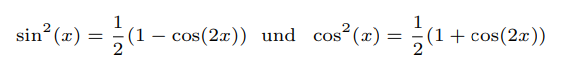
\includegraphics[scale=0.5]{Analysis1/zsf/Images/Basics/potenz_winkelfunktion.png}
\end{corollary}
\begin{corollary}{Eigenschaften mit $\pi$}
    \begin{enumerate}[itemsep= 2pt]
        \item $e^{i\pi} = -1, \quad e^{2i\pi} = 1$
        \item $\sin\left(x + \frac{\pi}{2}\right) = \cos(x), \quad \cos\left(x + \frac{\pi}{2}\right) = -\sin(x)$
        \item $\sin(x+\pi) = -\sin (x), \quad \sin(x + 2\pi) = \sin(x)$
        \item $\cos(x+\pi) = -\cos (x), \quad \cos(x + 2\pi) = \cos(x)$
    \end{enumerate}
\end{corollary}
\begin{corollary}{Nullstellen}
    \begin{enumerate}
         \item $\text{Nullstellen Sinus} = \{k\cdot \pi : k\in \mathbb{Z}\}$\\
        $\sin(x) > 0 \quad \forall x \in ]2k\pi, ~(2k+1)\pi[, ~ k\in \mathbb{Z}$\\[2pt]
        $\sin(x) < 0 \quad \forall x \in ](2k + 1)\pi, ~(2k+2)\pi[, ~ k\in \mathbb{Z}$
        \item $\text{Nullstellen Cosinus} = \left\{\frac{\pi}{2}+k\cdot \pi : k\in \mathbb{Z}\right\}$\\
        $\cos(x) > 0:\forall x \in \left]-\frac{\pi}{2} +2k\pi, ~-\frac{\pi}{2} +(2k+1)\pi\right[, ~ k\in \mathbb{Z}$\\[2pt]
        $\cos(x) < 0:\forall x \in \left]-\frac{\pi}{2} + (2k + 1)\pi, ~-\frac{\pi}{2} +(2k+2)\pi\right[, ~ k\in \mathbb{Z}$
    \end{enumerate}
\end{corollary}
\noindent Für $\tan(x)$ gilt $x \notin \frac{\pi}{2} + \pi \cdot \Z$ \qquad Für $\cot(x)$ gilt $x \notin \pi \Z$



                \raggedcolumns
                \columnbreak
                \subsubsection{Logarithmen}
\begin{corollary}{Natürlicher Logarithmus}
   Der nat. Logarithmus $\ln:]0, + \infty[ \to \R$ ist eine streng monoton wachsende, stetige, bijektive Funktion. 
\end{corollary}
\begin{corollary}{Rechnen mit Logarithmen}
    \begin{enumerate}
        \item Für $a > 0$ ist $]0, \infty[ \to ]0 + \infty[$ \quad $x \mapsto x^a$ eine stetige, streng monoton wachsende Bijektion.
        \item Für $a < 0$ ist $]0, \infty[ \to ]0 + \infty[$ \quad $x \mapsto x^a$ eine stetige, streng monoton fallende Bijektion.
        \item $\ln (a \cdot b) = \ln a + \ln b \quad \forall a,b \in ]0 +  \infty[$
        \item $\ln (a \div b) = \ln a - \ln b \quad \forall a,b \in ]0 +  \infty[$
        \item ${\ln \left(x^a\right) = a \ln (x) \quad \forall a \in \R, \forall x > 0}$
        \item ${x^a \cdot x^b = x^{a+b} \quad a,b \in \R, \forall x > 0}$
        \item ${\left(x^a\right)^b = x^{a \cdot b} \quad \forall a,b \in \R, \forall x > 0}$
    \end{enumerate}
    Im Allgemeinen gilt: $log_b (a) = \frac{ln(a)}{ln(b)}$
\end{corollary}
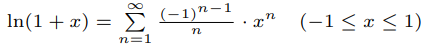
\includegraphics[scale=0.5]{Analysis1/zsf/Images/Basics/ln.png}
\subsubsection{Werte von log}
\begin{equation*}
	\begin{array}{lccccccc}
		& 0 & 1 & 2 & e & 3 & 5 & 10\\
		\ln & - \infty & 0 & 0.693 & 1 & 1.09 & 1.609 & 2.303\\
		\log_2 & - \infty & 0 & 1 & 1.443 & 1.585 & 2.321 & 3.321\\
		\log_{10} & - \infty & 0 & 0.301 & 0.434 & 0.477 & 0.699 & 1
	\end{array}
\end{equation*}

                \subsubsection{Relle Exponentialfunktion}
\begin{center}
    \hfill
    \begin{minipage}{0.3\linewidth}
        \begin{iequation}
            \exp (z) \coloneqq \sum_{n=0}^\infty \frac{z^n}{n!}
        \end{iequation}
    \end{minipage}
    \hfill
    \begin{minipage}{0.6\linewidth}
        \begin{theorem}{Eigenschaften}
            $\exp : \R \to ]0, + \infty[$ ist streng monoton wachsend, stetig und surjektiv.
        \end{theorem}       
    \end{minipage}
    \hfill
\end{center}

%\begin{center}
    \begin{minipage}{0.5\linewidth}
        \begin{iequation}[align*]
            \exp(-x)\exp(x) &= 1\\
	    \text{\textbf{\textsf{}}} \quad\exp(x) &> 0 \qquad\forall x \in \R \tikz[remember picture, overlay]
	    \coordinate(expineq) at (0,0);\\
            \exp(x) &> 1 \qquad\forall x > 0\\
            \exp(a+b) &= \exp(a) \cdot \exp(b)\\ 
            \exp(a-b) &= \exp(a) \div \exp(b)
        \end{iequation}
\begin{tikzpicture}[overlay, remember picture]
	\node[overlaynote, above right = 8mm and 0mm of expineq] (expineqnote) {Aber nicht: $\exp(z) > 0 \quad \forall z \in \C$};
\end{tikzpicture}
    \end{minipage}
    \hfill
    \begin{minipage}{0.48\linewidth}
        \begin{corollary}
            \\$\exp(z) > \exp(y) \quad \forall z > y$
        \end{corollary}
        \begin{corollary}
            \\${\exp (x) \geq 1 + x \quad \forall x \in \R}$
        \end{corollary}    
        \begin{corollary}
            \\$e^{\alpha x} = \sum_{n=0}^\infty \frac{\alpha^n x^n}{n!}$
        \end{corollary}
    \end{minipage}
%\end{center}
$\exp(z) = \exp(y + (z-y)) = \exp(y) \exp(z-y)\\
            \exp(x) = \lim_{n\to \infty}(1 + \frac{x}{n})^n$\\
 \begin{minipage}{0.6\linewidth}
        \begin{align*}
            \exp(\ln a + \ln b) &= \exp(\ln a) \cdot \exp (\ln b)\\
            \exp(\ln a)\exp(\ln b) &= ab = \exp(\ln ab)\\
            \exp(\ln a + \ln b) &= \exp(\ln ab)\\
            \ln a + \ln b &= \ln (ab)
        \end{align*}
    \end{minipage}
    \hfill
    \begin{minipage}{0.35\linewidth}
        \begin{iequation}
            x^a \coloneqq \exp(a \ln x)
        \end{iequation}
    \end{minipage}





                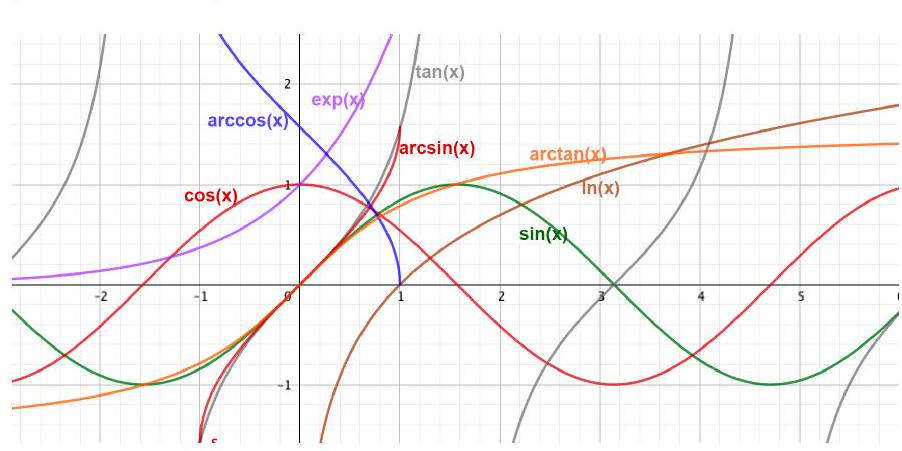
\includegraphics[scale=0.25]{Analysis1/zsf/Images/Basics/2024_01_21_1db6371ff954f8425d2dg-10.jpg}
                

        \raggedcolumns
        \columnbreak
        
        \section{Folgen und Reihen}
            \subsection{Folgen}
            \begin{definition}{Folgen}
    \begin{itemize}
  \item $n \in \mathbb{N}^{*} \rightarrow a_{n} \in \mathbb{R}$
  \item $\left(a_{k}\right)=\left(a_{k}\right)_{k \geq 1}=\left(a_{1}, a_{2}, a_{3}, \ldots, a_{n}, a_{n-1}, \ldots\right)$
\end{itemize}

Die Elemente einer Folge heissen Glieder der Folge $\rightarrow a_{n}$.
\end{definition}

\begin{definition}{Teilfolgen}
    Eine \emph{Teilfolge} einer Folge $\sequence$ ist eine Folge $\sequence[b]$ wobei $b_n = a_{l(n)}$ und $l: \N^* \to \N^*$ eine Abbildung mit der Eigenschaft: $l(n) < l(n+1)~\forall n \geq 1$.
\end{definition}

\begin{definition}{Monotonie}
    \begin{enumerate}
        \item $\sequence$ \emph{monoton wachsend} falls: \null\hfill $a_n \leq a_{n + 1} \quad \forall n \geq 1$.
    	\item $\sequence$ \emph{monoton fallend} falls: \null\hfill $a_n \geq a_{n+1} \quad \forall n \geq 1$.
    \end{enumerate}
\end{definition}
            \begin{formula}{Wichtige Folgen}\\
    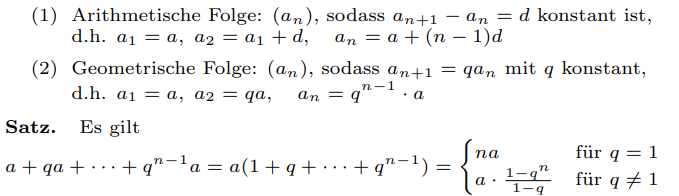
\includegraphics[scale=0.5]{Analysis1/zsf/Images/Folgen_Reihen/wichtige_folgen.png}
\end{formula}
\begin{remark}
    Folgend sind diese Konzepte beispielhaft vereinfacht.\\
    Abkürzungen
    \begin{itemize}
      \item $A=$ Anfangs-Glied
      \item $d=$ Differenz
      \item $q=$ Quotient
    \end{itemize}
\end{remark}

\begin{definition}{Arithmetische Folge}
$$
a_{k}=(2,3,4,5, \ldots) \rightarrow d=1, A=2
$$

N-tes Glied

$$
a_{n}=A+(n-1) \cdot d
$$

Mittelwert

$$
a_{k}=\frac{a_{k-1}+a_{k+1}}{2}
$$

Partial-Summe

$$
S_{n}=n \cdot \frac{a_{1}+a_{n}}{2}=n \cdot\left(A+\frac{n-1}{2} \cdot d\right)
$$
\end{definition}

\begin{definition}{Geometrische Folge}
$$
a_{k}=\left(\frac{1}{1}, \frac{1}{2}, \frac{1}{4}, \frac{1}{8}, \ldots\right) \rightarrow q=\frac{1}{2}, A=1
$$

N-tes Glied
$$a_{n}=A \cdot q^{n-1}=\frac{A}{q} \cdot q^{n}$$

Mittelwert
$$
\left|a_{k}\right|=\sqrt{a_{k-1} \cdot a_{k+1}}
$$

Partial-Summe

$$
S_{n}=A \cdot \frac{1-q^{n}}{1-q}=A \cdot \frac{q^{n}-1}{q-1}
$$
\end{definition}
            \subsection{Grenzwert und Konvergenz von Folgen}
    		  

\begin{definition}{$\varepsilon$-Definition}
    \\Folge $\sequence$ heisst \emph{konvergent}, falls es $l \in \R$ gibt, sodass \vspace{1mm}
    
    $\forall \varepsilon > 0$ die Menge $\{n \in \N^* : a_n \notin~] l - \varepsilon, l + \varepsilon[\,\}$ endlich ist. ($\N^*$: $\N$/$0$.) \vspace{1mm} \\ 
    Einfach gesagt: das heisst, dass $|a_n - a| < \epsilon$ ab einem gewissen n für alle $\epsilon$ gilt.
   
\end{definition}
Bem: $l$ bezeichnet den Grenzwert $\lim_{n \to \infty} a_n$
\begin{definition}{Formelle Grenzwert Definition}
    Folgende Aussagen sind äquivalent:
    \begin{enumerate}
        \item $\sequence$ konvergiert gegen $l = \lim_{n \to \infty} a_n$
        \item $\forall \varepsilon > 0~\exists N \geq 1$, sodass $|a_n -l | < \varepsilon \quad \forall n \geq N$.
    \end{enumerate}
\end{definition}
\begin{lemma}{Einzigartigkeit Grenzwert}
     Es gibt max. ein $l \in \R$ für $a_n$ mit dieser Eigenschaft (max. 1 Grenzwert)
\end{lemma}
\begin{theorem}{Rechenregeln mit Folgen}
    \\Sei $\sequence,\sequence[b]$ konvergente Folgen mit$a = \lim_{n \to \infty} a_n$, $b = \lim_{n \to \infty} b_n$
    \begin{enumerate}
        \item $(a_n \pm b_n)_{n \geq 1}$ konvergent, $\lim_{n \to \infty} (a_n \pm b_n) = a \pm b$.
        \item $(a_n \cdot b_n)_{n \geq 1}$ konvergent, $\lim_{n \to \infty} (a_n \cdot b_n) = a \cdot b$.
        \item $(a_n \div  b_n)_{n \geq 1}$ konvergent, $\lim_{n \to \infty} (a_n \div b_n) = a \div b$.
        \\(solange $b_n \neq 0 ~ \forall n \geq 1$ und $b \neq 0$)
        \item Falls $\exists K \geq 1$ mit $a_n \leq b_n ~ \forall n \geq K$ folgt $a \leq b$.
    \end{enumerate}
\end{theorem}






                \subsubsection{Tricks und Tipps für Folgen}
                \graphicspath{./Images}


\begin{KR}{Konvergenz Folgen}
    \begin{enumerate}
        \item Für Brüche, grösste Potenz von n ausklammern und kürzen. Alle übrigen Brüche der Form $\frac{a}{n^s}$ streichen, da diese zu 0 konvergieren.
        \item Für Wurzeln in einer Summe, multipliziere mit der Differenz der Summe (bei a + b multipliziere mit a - b)
        \item Anwendung Satz von Weierstrass
        \item Anwendung Sandwich-Satz 
        \item Vergleich mit Referenz-Folgen (Spezielle Grenzwerte)
        \item Grenzwert durch simple Operationen und Umformen ermitteln
        \item Binom -, Substitutions-, Log-Trick?
        \item Definition der Konvergenz/Limes anwenden
        \item Suchen eines konvergenten Majoranten
    \end{enumerate}
\end{KR}
\begin{KR}{Divergenz Folgen}
    \begin{enumerate}
        \item  Suche einen divergenten Minoranten
        \item Für alternierende Folgen zeige, dass \\$\lim_{n \to \infty} a_p1(n) \neq \lim_{n \to \infty} a_p2(n)$
    \end{enumerate}
\end{KR}

    







                \begin{KR}{Binom Trick}\\
    
\includegraphics[scale=0.5]{Analysis1/zsf/Images/Folgen_Reihen/binomtrick.png}
\end{KR}
\begin{KR}{Substitutions Trick}\\
    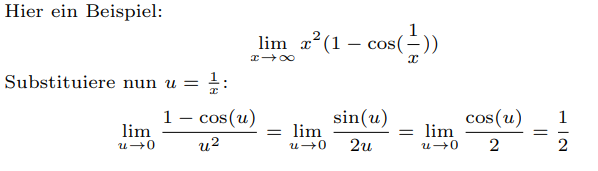
\includegraphics[scale=0.5]{Analysis1/zsf/Images/Folgen_Reihen/substitutionstrick.png}
\end{KR}
                \graphicspath{}
\begin{highlight}{Spezielle Grenzwerte von Folgen}
    \tcbsubtitle{$n \to \infty$}
    \begin{equation*}
        n^x q^n \to 0 \quad \forall x \in \Z~\text{und}~0 \leq q \leq 1
    \end{equation*}
    \begin{equation*}
         n(\sqrt[n]{x} - 1) \to \ln x \quad \forall x>0
    \end{equation*}
    \begin{equation*}
        \sqrt[n]{a_n} \to 1 ~\text{wenn}~ \lim_{n \to \infty} a_n > 0 ~\text{und}~ \forall a_n > 0 
    \end{equation*}
    \begin{center}
        \begin{minipage}{0.3\linewidth}
            \begin{align*}
                \frac{1}{n} &\to 0\\
                1 + \frac{1}{n} &\to 1\\
                \frac{2n}{2^n} &\to 0\\
                \sqrt[n]{n} = n^{\frac{1}{n}} &\to 1\\
                \sqrt[n]{n!} &\to \infty\\
                \frac{1}{n}\sqrt[n]{n!} &\to \frac{1}{e}\\
                \frac{x^n}{n!} &\to 0\\
                \frac{n^n}{n!} &\to \infty
            \end{align*}
        \end{minipage}
        \hfill\vline\hfill
        \begin{minipage}{0.3\linewidth}
            \begin{align*}
                % \frac{a^n}{n!} &\to 0\\
                % \left(\frac{n+1}{n}\right)^n &\to e\\
                e^n &\to \infty\\
                e^{-n} &\to 0\\
                \frac{e^n}{n^x} &\to \infty\\
                \frac{\sin n}{n} &\to 0\\
                \arctan n &\to \frac{\pi}{2}\\
                ln(n) &\to \infty\\
                \frac{ln(n)}{n} &\to 0\\
                \frac{log(n)}{n - 1} &\to 1
            \end{align*}
        \end{minipage}
        \hfill\vline\hfill
        \begin{minipage}{0.3\linewidth}
            \begin{align*}
                \forall k \in \Q^+ \hspace{2mm}\frac{1}{n^k} &\to 0\\
                \left(1 + n\right)^{\frac{1}{n}} &\to 1\\
                \left(1 + \frac{1}{n}\right)^x &\to 1\\
                \left(1 + \frac{1}{n}\right)^n &\to e\\
                \left(1 + \frac{x}{n}\right)^n &\to e^x\\
                \left(1 - \frac{1}{n}\right)^n &\to \frac{1}{e}\\
                \left(\frac{n}{n + x}\right)^n &\to e^{-x}
                % \left(1 - \frac{x}{n}\right)^n &\to e^{-x}\\
                % \binom{a}{n} &\to 0 \quad\text{für}~a > -1
            \end{align*}
        \end{minipage}
    \end{center}
    \begin{comment}
    \tcbsubtitle{$n \to 0$}
     \begin{minipage}{0.3\linewidth}
        \begin{align*}
            \ln n &\to -\infty\\
            \frac{ln(n+1)}{n} &\to 1\\
            n \log n &\to 0\\
            \frac{\log 1 - n}{n} &\to -1\\
            \frac{\log 1 - n}{n} &\to -1\\
            \forall x>0 \hspace{1mm}\frac{x^n-1}{n} &\to \ln(x)
        \end{align*}
    \end{minipage}
    \hfill\vline\hfill
    \begin{minipage}{0.3\linewidth}
        \begin{align*}
            \frac{\sin n}{n} &\to 1\\
            \frac{\cos n - 1}{n} &\to 0\\
            \frac{1}{\cos n} &\to 1\\
            \frac{1 - \cos n}{n^2} &\to \frac{1}{2}
        \end{align*}
    \end{minipage}
    \hfill\vline\hfill
    \begin{minipage}{0.3\linewidth}
        \begin{align*}
            \frac{1}{\arctan n} &\to 1\\
            \frac{e^n - 1}{n} &\to 1\\
            \frac{e^an - 1}{n} &\to a\\
            \left(1 + n\right)^{\frac{1}{n}} &\to e
        \end{align*}
    \end{minipage}
    \tcbsubtitle{Weitere Grenzwerte}
     \begin{minipage}{0.3\linewidth}
        \emph{$n \to -\infty$}
        \begin{align*}
            e^n &\to 0\\
            e^{-n} &\to \infty\\
            ne^n &\to 0
        \end{align*}
        \emph{$n \to 0+$}
        \begin{align*}
            n \ln n &\to 0
        \end{align*}
    \end{minipage}
    \hfill\vline\hfill
    \begin{minipage}{0.3\linewidth}
        \emph{$n \to \pm\infty$}
        \begin{align*}
            \left(1 + \frac{1}{n}\right)^n &\to e\\
            \left(1 + \frac{x}{n}\right)^an &\to e^ax
        \end{align*}
    \end{minipage}
    \hfill\vline\hfill
    \begin{minipage}{0.3\linewidth}
    \emph{$n \to \frac{\pi-}{2}$}
        \begin{align*}
            \tan x &\to +\infty
        \end{align*}
    \emph{$n \to \frac{\pi+}{2}$}
        \begin{align*}
            \tan x &\to -\infty
        \end{align*}
    \end{minipage}
    \end{comment}
    \tcbsubtitle{Divergente Folgen}
    \begin{align*}
        &a_{n}=(-1)^{n}=(-1,1,-1,1,-1 \ldots) \\
        &a_{n}=3+2 n=(5,7,9,11, \ldots)
    \end{align*}
\end{highlight}



                
\begin{definition}{Supremum und Infimum}
    $A \subseteq \R, ~A\neq \emptyset$
    \begin{enumerateroman}
        \item $A$ nach oben beschränkt. Dann gibt es eine kleinste obere Schranke von $A$: $c \coloneqq \sup A$. Das \emph{Supremum} von $A$.
        \item $A$ nach unten beschränkt. Dann gibt es eine kleinste untere Schranke von $A$: $c \coloneqq \inf A$. Das \emph{Infimum} von $A$.
    \end{enumerateroman}
    \tcblower 
    Vereinfacht formuliert: Für ein abgeschlossenes, halboffenes oder offenes Intervall $[a,b], [a,b), (a,b]$ oder $(a,b)$ gilt $inf = a$, $sup = b$ (solange $a, b \neq \infty$)
\end{definition}

\begin{concept}{Satz von Weierstrass}
    \begin{itemize}
        \item $\sequence$ monoton wachsend und nach oben beschränkt. $\Rightarrow$ $\sequence$ konvergiert mit $\lim_{n \to \infty} a_n = \sup \{a_n : n \geq 1\}$
        \item $\sequence$ monoton fallend und nach unten beschränkt. $\Rightarrow$ $\sequence$ konvergiert mit $\lim_{n \to \infty} a_n = \inf \{a_n : n \geq 1\}$
    \end{itemize}
\end{concept}

\begin{theorem}{Sandwich-Satz}
    Sei $\lim a_n = \alpha$ und $\lim c_n = \alpha$ und $a_n \leq b_n \leq c_n, \forall n \geq k$ dann gilt $\lim b_n = \alpha$\\
    Bmk: k steht hier für eine beliebige natürliche Zahl, ab der die Bedingung immer gilt. Also wie bei der Grenzwert-Definition mit dem <<Gürtel>> um den Grenzwert - das gilt ja auch erst ab einem gewissen Wert n.\\
    Bmk 2: Einfach gesagt heisst das, dass wenn wir den Grenzwert von zwei Folgen bereits kennen und dieser für beide gleich ist, und wir eine dritte Folge haben die <<zwischen>> die zwei bekannten Folgen passt (daher Sandwich-Satz), wissen wir dass auch die dritte Folge den gleichen Grenzwert wie die anderen zwei hat.
\end{theorem}    




                

                \raggedcolumns
                \columnbreak
                
                
            \subsection{Grenzwert einer Reihe}
		      
\begin{definition}{Reihen-Konvergenz}
    Die Reihe $\sum_{k = 1}^\infty a_k$ ist \emph{konvergent}, falls die Folge $\sequence[S]$ der Partialsummen konvergiert. In diesem Fall definieren wir: $\sum_{k = 1}^\infty a_k \coloneqq \lim_{n \to \infty} S_n$
    % \begin{equation*}
    %     \sum_{k = 1}^\infty a_k \coloneqq \lim_{n \to \infty} S_n
    % \end{equation*}
\end{definition}
\begin{theorem}{Rechenregeln von Reihen}
    \\Seien $\sum_{k=1}^\infty a_k$ und $\sum_{j=1}^\infty b_j$ konvergent, sowie $\alpha \in \C$.
    \begin{enumerate}
        \item Dann ist $\sum_{k=1}^\infty (a_k + b_k)$ konvergent.\\
            $\sum_{k=1}^\infty (a_k + b_k) = (\sum_{k=1}^\infty a_k) + (\sum_{j=1}^\infty b_j)$.
        \item Dann ist $\sum_{k=1}^\infty \alpha a_k$ konvergent. $\sum_{k=1}^\infty \alpha a_k = \alpha \sum_{k=1}^\infty a_k$
    \end{enumerate}
\end{theorem}










                
            
                
                


\begin{highlight}{Spezielle Grenzwerte von Reihen}\\
	\begin{array}{lcl}
		\text{Geom:} & \sum_{k = 0}^\infty a^k & \begin{cases}
		    \frac{1}{1 - a} & |a| < 1\\
		    \text{divergiert} & |a| \geq 1
		\end{cases}\\[10pt]
		& \sum_{k=0}^n ax^k & = a (\frac{1 - x^{n+1}}{1-x})\\[5pt]
		\text{Harm. mit}~b= 1 & \sum_{k = 1}^\infty \frac{1}{k^b} & \begin{cases}
		    \text{konvergiert} & b > 1\\
		    \text{divergiert} & b \leq 1
		\end{cases}\\[10pt]
		\text{Altern. Harm.} & \sum_{k = 1}^\infty \frac{(-1)^{n+1}}{k^b} & \text{konvergiert nach Leibniz}\\[10pt]
		& \sum_{k = 1}^\infty \frac{k^a}{b^k} & \text{abs. konv. falls}~ |b| > 1, k \in \C\\[10pt]
		& \sum_{k = 1}^\infty \frac{k^a}{k!} & \text{abs. konv.}~\forall a \in \C\\[10pt]
	\end{array}
\end{highlight}

\emph{Zeta-Funktion}:
Sei $s > 1$ und $\zeta (s) = \sum_{n=1}^\infty \frac{1}{n^s}$. $\zeta(s)~\text{konvergiert für}~ s> 1$\\
\emph{Teleskopsumme}: Sei $\sum_{k=1}^\infty (a_k - a_{k-1})$. Konvergiert genau dann, wenn $\lim a_n \to g$ konvergiert. Der Grenzwert der Summe ist dann $a_1 -g$.

                \begin{formula}{Die unendliche Geometrische Reihe}
    $$
    S=\sum_{k=1}^{\infty} A q^{k-1}=\frac{A}{1-q}
    $$
    
    Bedingung
    
    $$|q|<1$$
\end{formula}

\begin{example2}{Beispiel Unendliche Geometrische Reihe}

$$
a_{k}=\frac{7}{2^{k-1}}=7+\frac{7}{2}+\frac{7}{4}+\frac{7}{8} \ldots=14
$$

\begin{itemize}
  \item $q=\frac{1}{2} \rightarrow$ Die Reihe konvergiert
  \item $S=\frac{A}{1-q}=\frac{7}{1-\frac{1}{2}}=14$
\end{itemize}
\end{example2}
                
\begin{corollary}{Reihen - Funktionen}\\
    \begin{array}{ll}
        \sum^{n}_{k=1} k = \frac{n \cdot (n+1)}{2} & \sum^{n}_{k=1} (2k - 1)^2 = \frac{n \cdot (4n^2-1)}{3}\\
    	\sum^{n}_{k=1} 2k-1 = n^2 & \sum^{n}_{k=1} k^3 = \left( \frac{n \cdot (n+1)}{2}\right)^2\\
    	\sum^{n}_{k=1} 2k = n(n+1) & \sum^{n}_{k=1} \frac{1}{k(k+1)} = \frac{n}{n+1}\\
    	\sum^{n}_{k=1} k^2 = \frac{n \cdot (n+1) \cdot (2n+2)}{6} &
    \end{array}
\end{corollary}








                \subsubsection{Konvergenzkriterien Reihen}
                
\begin{KR}{Konvergenz Reihen}
    \begin{enumerate}
        \item Handelt es sich um eine spezielle Reihe? (Geometrisch, Teleskopiert, Harmonisch, Zetafunktion)
        \item Ist $\lim a_n$ = 0? (Nullfolgenkriterium)
        \item Ist das Quotientenkriterium oder Wurzelkriterium anwendbar?
        \item Existiert ein konvergierender Majorant / divergirender Minorant?
        \item Kann man das Leibnitzkriterium anwenden?
        \item Integral Test? Partialbruchzerlegung?
    \end{enumerate}
\end{KR}

    

\begin{center}
    \begin{tikzpicture}[font = \footnotesize]
        \node[draw] (origin) {Gegeben: $\sum_{n=0}^\infty a_n$};
        \matrix (stypes) [
            below = 5mm and 2mm of dstype,
            column sep = 2mm,
            nodes = {
                rectangle, 
                draw,
                text width = 18mm,
                minimum height = 12mm
            }
        ] {
            \node[label={[label distance = -4mm]270:geom. Reihe}] (stype1) {$\sum q^n$\\[5pt] $|q| < 1$}; & 
            \node[label={[label distance = -4mm]270:altern. Reihe}] (stype2) {$\sum (-1)^n a_n$\\[5pt] $\lim a_n = 0$}; &
            \node[label={[label distance = -4mm]270:Riemann Zeta}] (stype3) {$\zeta (s) = \sum\limits_{n=1}^\infty \frac{1}{n^s}$\\ $s > 1$}; & 
            \node[label={[label distance = -4mm]270:Teleskop-Reihe}] (stype4) {$\sum (a_n - a_{n-1})$ \\[5pt] $\exists \lim a_n$}; \\
        };
    \end{tikzpicture}
\end{center}


                
                \begin{concept} {Nullfolgenkriterium}\\
    $\sum_{k=1}^\infty a_k~\text{konvergiert} \Rightarrow \lim_{k \to \infty} a_k = 0$ aber die Umkehrung stimmt nicht.
\end{concept}
\begin{concept} {Cauchy Kriterium}\\
    Die Reihe $\sum_{k=1}^\infty a_k$ ist genau dann konvergent, falls:\\
    $\forall \varepsilon > 0 ~\exists N \geq 1$ mit $\left|\sum_{k=n}^m a_k \right| < \varepsilon \quad \forall m \geq n \geq N$
\end{concept}
\begin{concept} {Leibniz Kriterium}\\
    Sei $\sequence$ monoton fallend, mit $a_n \geq 0~\forall n \geq 1$ und $\lim_{n \to \infty} a_n = 0$. Dann konvergiert\\
    $S \coloneqq \sum_{k = 1}^{\infty} (-1)^{k+1} a_k$
    und es gilt: $a_1 - a_2 \leq S \leq a_1$.
\end{concept}
\begin{concept} {Majorantenkriterium}\\
    Seien $a_n, b_n \geq 0$ mit $a_n \geq b_n \quad \forall n > n_0$:\\
    $\sum_{n=0}^\infty a_n$ konvergiert $\Rightarrow \sum_{n=0}^\infty b_n$ konvergiert 
\end{concept}
\begin{concept} {Minorantenkriterium}\\
    Seien $a_n, b_n \geq 0$ mit $a_n \leq b_n \quad \forall n > n_0$:\\
    $\sum_{n=0}^\infty a_n$ divergiert $\Rightarrow \sum_{n=0}^\infty b_n$ divergiert 
\end{concept}
\begin{concept} {Quotientenkriterium}\\
    Sei $\sequence$ mit $a_n \neq 0~\forall n \geq 1$ und: $q = \frac{|a_{n + 1}|}{|a_n|}$\\
    Falls:
    \begin{itemize}
        \item $q < 1$ konvergiert $\sum_{n=1}^\infty a_n$ absolut
        \item $q > 1$ divergiert $\sum_{n=1}^\infty a_n$
    \end{itemize}
    Für $\liminf a_n = 1$ keine Aussage möglich\\
    \emph{!!! für die harmonische Reihe ist dieses Kriterium nicht anwendbar/gültig !!!}
\end{concept}
\begin{concept} {Wurzelkriterium}\\
    Es sei: $q = \sqrt[n]{|a_n|}$\\
    Dann gilt:
    \begin{itemize}
        \item $q < 1 \Rightarrow \sum_{n=1}^\infty a_n$ konvergiert 
        \item $q > 1 \Rightarrow \sum_{n=1}^\infty a_n$ und $\sum_{n=1}^\infty |a_n|$ divergieren
        \item $q = 1 \Rightarrow$ keine Aussage möglich
    \end{itemize}
\end{concept}
\begin{KR}{Logarithmus abschätzen}\\
    $\log_b (n)$ kann mit $n^\alpha$ ($\alpha > 0$) abgeschätzt werden.\\
    $\ln(n) \leq \sqrt{n}$
\end{KR} 
\begin{KR}{Integral Test}\\
    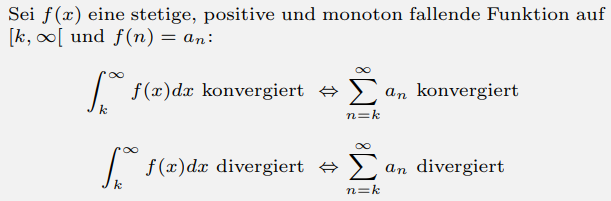
\includegraphics[scale=0.5]{Analysis1/zsf/Images/Folgen_Reihen/integraltest.png}
\end{KR}
               \noindent Der Grenzwert einer Reihe kann auch mit Partialbruchzerlegung berechnet werden.
\begin{example}
    Was ist der Grenzwert von $\sum_{n=1}^\infty \frac{2}{(n+1)(n+3)}$?
    \tcblower
    \begin{equation*}
        \frac{2}{(n+1)(n+3)} = \frac{a}{n+1} + \frac{b}{n+3} \Rightarrow \begin{cases}
            a + b = 0\\
            3a - b = 2
        \end{cases}
        \quad
        \begin{matrix}
            b = -a = -\frac{1}{2}\\
            a = \frac{1}{2}
        \end{matrix}
    \end{equation*}
    \begin{align*}
        \Rightarrow \sum_{n=1}^\infty \frac{2}{(n+1)(n+3)} &= \frac{1}{2}\sum_{n=1}^\infty\left(\frac{1}{n+1} - \frac{1}{n+3}\right)\\
        & = \frac{1}{2}\left(\frac{1}{2} - \cancel{\frac{1}{4}} + \frac{1}{3} - \cancel{\frac{1}{5}} + \cancel{\frac{1}{4}} - \cancel{\frac{1}{6}} + \ldots\right)\\
        &= \frac{1}{2}\left(\frac{1}{2} + \frac{1}{3}\right) = \frac{5}{2 \cdot 6} = \frac{5}{12}
    \end{align*}
\end{example}
                   
                \raggedcolumns
                \columnbreak

                \section{Funktionen}
                    \begin{center}
    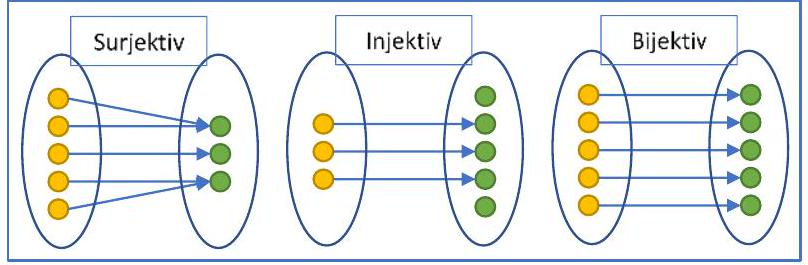
\includegraphics[scale=0.2]{Analysis1/zsf/Images/Stetige_Funktionen/2024_01_20_7bfda6c084929ccc01ffg-01(3).jpg}
\end{center}


\begin{definition}{Umkehrfunktion}
\begin{itemize}
  \item Bijektive Funktion $f: D \rightarrow W$
  \item Umkehrunktion $f^{-1} \quad g: W \rightarrow D$
\end{itemize}
Vorgehen $f(x)=y$:
\begin{itemize}
  \item Nach $x$ auflösen $\quad \rightarrow x=g(y)$
  \item Variablen vertauschen $\rightarrow y=g(x)$
\end{itemize}
\end{definition}



\begin{theorem}{Operationen von Funktionen}
    \begin{itemize}
  \item Addition $x \rightarrow f(x)+g(x)$
  \item Subtraktion $x \rightarrow f(x)-g(x)$
  \item Multiplikation $x \rightarrow f(x) \cdot g(x)$
    \item Division $x \rightarrow f(x) / g(x)$
\end{itemize}



\begin{itemize}
  \item Komposition/Verkettung: $(g \circ f)(x)=g(f(x))$
\end{itemize}
\end{theorem}

\begin{definition}{Symmetrie}
\begin{itemize}
  \item gerade $f(-x)=f(x)$
  \item ungerade $f(-x)=-f(x)$
\end{itemize}
\end{definition}

\begin{center}
    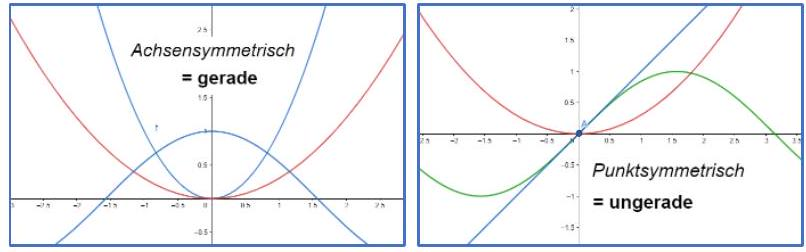
\includegraphics[scale=0.3]{Analysis1/zsf/Images/Stetige_Funktionen/2024_01_20_7bfda6c084929ccc01ffg-01(2).jpg}
\end{center}

\begin{definition}{Beschränktheit}
    Sei $f \in \R^D$.
    \begin{enumerate}
        \item $f$ ist \emph{nach oben beschränkt}, falls $f(D) \subseteq \R$ nach oben beschränkt.
        \item $f$ ist \emph{nach unten beschränkt}, falls $f(D) \subseteq \R$ nach unten beschränkt.
        \item $f$ ist \emph{beschränkt}, falls $f(D) \subseteq \R$ beschränkt.
    \end{enumerate}
\end{definition}

\begin{definition}{Monotonie}
    \begin{itemize}
  \item monoton wachsend $f\left(x_{1}\right) \leq f\left(x_{2}\right)$
  \item streng monoton wachsend $f\left(x_{1}\right)<f\left(x_{2}\right)$
  \item monoton fallend $f\left(x_{1}\right) \geq f\left(x_{2}\right)$
  \item streng monoton wachsend $f\left(x_{1}\right)>f\left(x_{2}\right)$
\end{itemize}
\end{definition}



                    \subsection{Stetigkeit}
                    \begin{definition}{Stetigkeit}
    Eine Funktion ist stetig, falls

    \begin{itemize}
      \item die Kurve keine Sprünge macht
      \item man den Graphen der Funktion zeichnen kann, ohne den Stift dabei abzusetzen
    \end{itemize}

\end{definition}

\begin{formula}{Spezielle Stetige Funktionen}
    \begin{enumerate}
        \item $|f|$, $max(f, g)$ und $min(f, g)$ sind stetig
        \item Polynomielle Funktionen sind auf ganz $\R$ stetig
        \item die Trigonometrischen Funktionen $sin : \R \to \R$ und $cos : \R \to \R$ sind stetig
        \item die Exponentialfunktion $e^x$ ist auf ganz $\R$ stetig
    \end{enumerate}
\end{formula}










                \subsection{Grenzwerte von Funktionen}
                    \noindent Für mehr wichtige/spezielle Grenzwerte, siehe Grenzwerte von Folgen.
\begin{highlight}{Wichtige Grenzwerte}
    \begin{center}
        \begin{minipage}{0.4\linewidth}
                \tcbsubtitle{Harmonische Folge:}
                $$\lim _{n \rightarrow \infty} \frac{1}{n}=0$$
                \tcbsubtitle{Geometrische Folge:}
                $$\lim _{n \rightarrow \infty} q^n=0 \quad(q<1)$$
        \end{minipage}
        \hfill\vline\hfill
        \begin{minipage}{0.5\linewidth}
            \tcbsubtitle{n-te Wurzel:}
            $$\lim _{n \rightarrow \infty} \sqrt[n]{a}=1$$
            \tcbsubtitle{Eulerzahl:}
            $$\lim _{n \rightarrow \infty}\left(1+\frac{1}{n}\right)^n=e$$
        \end{minipage}
    \end{center}
\end{highlight}

\begin{definition}{Konvergenz einer Funktion}\\
    Die Funktion $y = f(x)$ hat an der Stelle $x_0$ den Grenzwert $y_0$ falls:\\
    für jede Folge $\left(x_{n}\right)$ mit $\lim _{n \rightarrow \infty} x_{n}=x_{0}$ gilt $\lim _{n \rightarrow \infty} f\left(x_{n}\right)=y_{0}$\\
    Bmk: Die Stelle $x_{0}$ muss nicht im Definitionsbereich $D$ sein.
\end{definition}

\begin{definition}{Konvergenz/Divergenz}
    \begin{itemize}
  \item Konvergenz:
  Funktion mit Grenzwert $x \rightarrow \infty$
  \item Divergenz:
  Funktion ohne Grenzwert $x \rightarrow \infty$
  \item Bestimmte Divergenz:
  Funktion mit $\lim _{x \rightarrow \infty} f(x)= \pm \infty$
\end{itemize}
\end{definition}

\begin{definition}{Links- und Rechtsseitige Grenzwerte}\\
    Sei $f : D \to \R$ und $x_0 \in \R$. Wir nehmen an, $x_0$ ist ein Häufungspunkt.\\ Was vereinfacht heisst, dass die Funktion an dieser Stelle evtl. einen Sprung macht, da sich z.B. die Definition ändert. Beispiel:
    \begin{equation*}
            f(x) = \begin{cases}
                0 & x < 0\\
                1 & x \geq 0
            \end{cases}
        \end{equation*}
    Setze in diesem Beispiel $x_0 = 0$, und prüfe ob sich die Funktion von rechts und links dem selben Wert nähert bei $x_0$. (NEIN in diesem Bsp.)

    \emph{Formell:} Eine Funktion ist dann gleichmässig konvergent wenn für alle Werte der Funktion gilt

    $$\lim_{x \to x_0^+} f(x) = \lim_{x \to x_0^-} f(x)$$

    (Linksseitiger Grenzwert = Rechtsseitiger Grenzwert)
\end{definition}









                    \begin{corollary}{Rechnen mit Grenzwerten von Funktionen}
    \begin{itemize}
        \item $\lim_{x \to x_0} (f + g)(x) = \lim_{x \to x_0} f(x) + \lim_{x \to x_0} g(x)$
        \item $\lim_{x \to x_0} (f \cdot g)(x) = \lim_{x \to x_0} f(x) \cdot \lim_{x \to x_0} g(x)$
        \item Sei $f \leq g$, so ist $\lim_{x \to x_0} f(x) \leq \lim_{x \to x_0} g(x)$
        \item Falls $g_1 \leq f \leq g_2$ und $\lim_{x \to x_0} g_1(x) = \lim_{x \to x_0} g_2(x)$, so existiert $\lim_{x \to x_0} f(x) = \lim_{x \to x_0} g_1(x)$
    \end{itemize}
\end{corollary}

\begin{concept}{l'Hospital Kettenregel Trick}
    Seien $f,g : ]a,b[ \to \R$ differenzierbar mit \\ $g'(x) \neq 0 \quad \forall x \in ]a,b[$. Falls $\lim_{x \to b^-} f(x) = 0$, $\lim_{x \to b^-} g(x) = 0$ und $\lambda \coloneqq \lim_{x \to b^-} \frac{f'(x)}{g'(x)}$ existiert, folgt
    \begin{iequation}
        \lim_{x \to b^-} \frac{f(x)}{g(x)} = \lim_{x \to b^-}\frac{f'(x)}{g'(x)}
    \end{iequation}
    \tcblower
    \emph{Nur für $\lim_{x \to 0} \frac{f(x)}{g(x)} = \frac{\mlqq 0 \mrqq}{\mlqq 0 \mrqq}$ oder $\frac{\mlqq \infty \mrqq}{\mlqq \infty \mrqq}$ erlaubt.}
\end{concept}

\raggedcolumns
\columnbreak

\subsubsection{Strategien und Rechentricks}
\begin{KR}{Erweitern mit}
    $\left(\frac{1}{n^k}\right)$\\
    $k=$ höchste Potenz
\end{KR}
\begin{example}
Beispiel:
    $$
    \begin{aligned}
    \lim _{n \rightarrow \infty} \frac{3 n^2+2 n+1}{5 n^2+4 n+2} \Longrightarrow & \textcolor{pink}{\frac{\frac{1}{n^2}}{\frac{1}{n^2}}} \cdot \frac{3 n^2+2 n+1}{5 n^2+4 n+2} =\frac{\frac{3 n^2}{n^2}+\frac{2 n}{n^2}+\frac{1}{n^2}}{\frac{5 n^2}{n^2}+\frac{4 n}{n^2}+\frac{2}{n^2}} \\
    &= \frac{3+\frac{2}{n}+\frac{1}{n^2}}{5+\frac{4}{n}+\frac{2}{n^2}}=\frac{3+0+0}{5+0+0}
    \end{aligned}
    $$
\end{example}

\begin{KR}{Erweitern mit}
    $\left(\frac{1}{a^k}\right)$\\
$k=$ höchste Potenz \\
$a=$ grösste Basis
\end{KR}
\begin{example}
Beispiel:
    $$
    \begin{aligned}
    \lim _{n \rightarrow \infty} \frac{3^{n+1}+2^n}{3^n+2} \Longrightarrow &  \textcolor{pink}{\frac{\frac{1}{3^n}}{\frac{1}{3^n}}} \cdot \frac{3 \cdot 3^n+2^n}{3^n+2}=\frac{\frac{3 \cdot 3^n}{3^n}+\frac{2^n}{3^n}}{\frac{3^n}{3^n}+\frac{2}{3^n}} \\
    & = \frac{3+\frac{2^n}{3^n}}{1+\frac{2}{3^n}}=\frac{3+0}{1+0}
    \end{aligned}
    $$
\end{example}

\begin{KR}{Erweitern mit}
    $\sqrt{a(n)}+\sqrt{b(n)}$
\end{KR}
\begin{example}
Beispiel:
    $$
    \begin{aligned}
    &\lim _{n \rightarrow \infty} \sqrt{n^{2}+n}-\sqrt{n^{2}-2 n}\\
    &\Longrightarrow \textcolor{pink}{\frac{\sqrt{n^{2}+n}+\sqrt{n^{2}-2 n}}{\sqrt{n^{2}+n}+\sqrt{n^{2}-2 n}}} \cdot \frac{\sqrt{n^{2}+n}-\sqrt{n^{2}-2 n}}{1} \\
    &=\frac{\left(\sqrt{n^{2}+n}\right)^{2}-\left(\sqrt{n^{2}-2 n}\right)^{2}}{\sqrt{n^{2}+n}-\sqrt{n^{2}-2 n}}=\frac{3 n}{\sqrt{n^{2}+n}-\sqrt{n^{2}-2 n}}\\
    &=\frac{\frac{1}{n}}{\frac{1}{n}} \cdot \frac{3 n}{\sqrt{n^{2}+n}-\sqrt{n^{2}-2 n}} \frac{\frac{3 n}{n}}{\sqrt{\frac{1}{n^{2}} \cdot\left(n^{2}+n\right)}-\sqrt{\frac{1}{n^{2}} \cdot\left(n^{2}-2 n\right)}}\\
    &=\frac{3}{\sqrt{\frac{n^{2}+n}{n^{2}}}-\sqrt{\frac{n^{2}-n}{n^{2}}}}=\frac{3}{\sqrt{1+\frac{1}{n}}-\sqrt{1+\frac{1}{n}}}=\frac{3}{\sqrt{1}+\sqrt{1}}=\frac{3}{2}
    \end{aligned}
    $$
\end{example}

\begin{KR}{Erweitern zu}
    $\lim _{n \rightarrow \infty}\left(1+\frac{1}{5 n}\right)^{n}$
    $$
      \lim _{x \rightarrow \infty}\left(\left(\left(1+\frac{1}{x}\right)^{x}\right)^{a}\right)=e^{a}
    $$
\end{KR}
\begin{example}
Beispiel:
    $$
    \begin{aligned}
    &\lim _{x \rightarrow \infty}\left(1+\frac{2}{3 n}\right)^{4 n}
    =\left(\left(1+\frac{1}{\frac{3 n}{2}}\right)^{\frac{3 n}{2}}\right)^{a}=e^{a}=e^{\frac{8}{3}}\\
    &\text{Wir rechnen also:}\\
    & 4 n=\frac{3 n}{2} \cdot a \text{ und } a=\frac{4 n}{\frac{3 n}{2}}=\frac{8}{3}
    \end{aligned}
    $$
\end{example}



   
    



                    \raggedcolumns
                    \columnbreak

                \section{Differentialrechnung}
                        \subsubsection{Differenzierbarkeit}
                        
\begin{definition}{Sekanten-Steigung und Differentialquotient}\\
    Sei $f$ eine Funktion und $\left[x_{0}, x_{0}+h\right]$ ein Intervall im Definitionsbereich von $f$. Der Quotient
    
    $$\frac{\Delta f}{\Delta \mathrm{x}}=\frac{f\left(x_{0}+h\right)-f\left(x_{0}\right)}{h}$$
    
    heisst Differentialquotient von $f$.
\end{definition}

\begin{center}
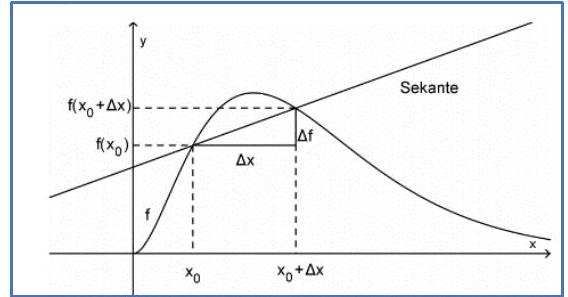
\includegraphics[scale=0.3]{Analysis1/zsf/Images/Differential/2024_01_20_7bfda6c084929ccc01ffg-03.jpg}
\end{center}

\begin{definition}{Differenzierbarkeit}\\
    $f$ ist in $x_0$ \emph{differenzierbar}, falls der Grenzwert $\lim_{x \to x_0} \frac{f(x) -f(x_0)}{x -x_0}$
    existiert.\\
    Ist dies der Fall, wird der Grenzwert mit $f'(x)$ bezeichnet.
        $$
        f'(x_0) = \lim_{h \to 0}\frac{\Delta f}{\Delta \mathrm{x}} = \lim_{h \to 0}\frac{f(x_0 + h) -f (x_0)}{h}
        $$
    Den Grenzwert selbst bezeichnet man als Ableitung.
    \tcblower 
    Vereinfacht: Eine Funktion ist differenzierbar, falls die Kurve keine Knicke macht.
\end{definition}

\begin{formula}{Tangentengleichung}
    $$
    y=f^{\prime}\left(x_{0}\right) \cdot\left(x-x_{0}\right)+f\left(x_{0}\right)
    $$
\end{formula}

\begin{definition}{Stetige Differenzierbarkeit}
	Eine Funktion ist stetig differenzierbar, wenn sie differenzierbar ist und ihre Ableitungsfunktion stetig ist.
\end{definition}







                    
                                
\begin{definition}{n-fache Differenzierbarkeit}
	\begin{enumerate}
		\item Für $n \geq 2$ ist $f$ \emph{$n$-mal differenzierbar} in $D$ falls $f^{n-1}$ in $D$ differenzierbar ist. Dann ist $f^{(n)} \coloneqq \left(f^{(n-1)}\right)'$ und nennnt sich die $n$-te Ableitung von $f$.
		\item Die Funktion $f$ ist \emph{$n$-mal stetig differenzierbar} in $D$, falls sie $n$-mal differenzierbar ist und falls $f^{(n)}$ in $D$ stetig ist.
		\item Die Funktion $f$ ist in $D$ \emph{glatt}, falls sie $\forall n \geq 1$, $n$-mal differenzierbar ist. 
	\end{enumerate}
\end{definition}


\begin{itemize}
	\item $\exp$, $\sin$, $\cos$, $\sinh$, $\cosh$, $\tanh$ sind glatt auf $\R$
	\item Alle Polynome sind auf ganz $\R$ glatt
	\item $\ln : ]0, + \infty[ \to \R$ ist glatt
\end{itemize}

\begin{theorem}{Rechnen mit höheren Ableitungen}\\
	Sei $D \subseteq \R$, $n \geq 1$ und $f,g \to \R$ $n$-mal differenzierbar in $D$.
	\begin{enumerate}
		\item $f+g$ ist $n$-mal differenzierbar und $(f + g)^{(n)} = f^{(n)} + g^{(n)}$
		\item $f \cdot g$ ist $n$-mal differenzierbar und\\ $(f \cdot g)^{(n)} = \sum_{k=0}^n \binom{n}{k} f^{(k)} g^{(n-k)}$.
        \item $\frac{f}{g}$ ist n-mal differenzierbar falls $g(x) \neq 0, \forall x \in D$
        \item $(g \circ f)$ ist n-mal differenzierbar
	\end{enumerate}
\end{theorem}



 

                            \raggedcolumns
                            \columnbreak
                        
                        
        
                        \subsection{Ableitungen}
                            



\begin{concept}{Ableitungsregeln}
    Seien $f,g: D \to \R$  differenzierbar. Dann gelten:
    \begin{itemize}
        \item Summe/Differenz: $$(f + g)'(x) = f'(x) + g'(x)$$
        \item Produkt: $$(f \cdot g)'(x) = f'(x)g(x) + f(x)g'(x)$$
        \item Quotient: $$\left(\frac{f}{g}\right)'(x) = \frac{f'(x) g(x) - f(x) g'(x)}{g(x)^2}$$
        \item Kettenregel: $$(g \circ f)' (x) = g'(f(x)) f'(x)$$
        \item Umkehrfunktion: $$\left(f^{-1}\right)'(y_0) = \frac{1}{f'(x)}$$
        \item Potenz/Logarithmus 1: 
        $$(a^{f(x)})' = ln(a) \cdot a^{f(x)} \cdot f'(x)$$
        $$(f(x)^{g(x)})' = f(x)^{g(x)} \cdot (ln(f(x)) \cdot g(x))' =  f(x)^{g(x)} \cdot (ln(f(x)) \cdot g(x) \cdot \frac{f'(x)}{f(x)})$$
    \end{itemize}
    Bem. Für gerade $k$ gilt $\cosh (x)^{(k)}=\cosh (x)$ und für ungerade $k$ gilt $\cosh (x)^{(k)}=\sinh (x)$, analoges gilt für $\sinh$.
\end{concept}

\begin{formula}{Grundfunktionen der Ableitung}
    \begin{itemize}
        \item Potenz
    \end{itemize}

    $$
    f(x)=x^{n} \quad f^{\prime}(x)=n \cdot x^{n-1}
    $$
    
    \begin{itemize}
      \item Exponent
    \end{itemize}
    
    $$
    \begin{array}{ll}
    f(x)=a^{x} & f^{\prime}(x)=a^{x} \cdot \ln (a) \\
    f(x)=e^{x} & f^{\prime}(x)=e^{x}
    \end{array}
    $$
    
    \begin{itemize}
      \item Logarithmus
    \end{itemize}
    
    $$
    \begin{array}{ll}
    f(x)=\ln (x) & f^{\prime}(x)=\frac{1}{x} \\
    f(x)=\log _{a}(x) & f^{\prime}(x)=\frac{1}{\ln (a) \cdot x}
    \end{array}
    $$
\end{formula}


\begin{formula}{Ableitungen von geometrischen Funktionen}
    $$
    \begin{aligned}
    \arctan ^{\prime}(x) & =\frac{1}{1+x^{2}} \\
    \arcsin ^{\prime}(x) & =\frac{1}{\sqrt{1-x^{2}}} \\
    \arccos ^{\prime}(x) & =\frac{1}{\sqrt{1+x^{2}}}
    \end{aligned}
    $$
    
    \begin{itemize}
      \item Tangens
    \end{itemize}
    
    $$
    \begin{array}{ll}
    f(x)=\tan (x) & f^{\prime}(x)=1+\tan ^{2}(x)=\frac{1}{\cos ^{2}(x)} \\
    f(x)=\cot (x) & f^{\prime}(x)=-1-\cot ^{2}(x)=-\frac{1}{\sin ^{2}(x)}
    \end{array}
    $$
\end{formula}

\begin{center}
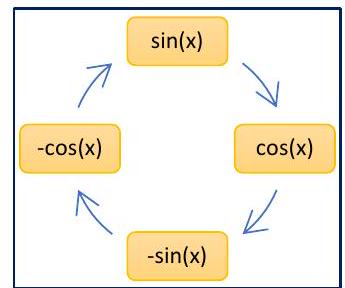
\includegraphics[scale=0.25]{Analysis1/zsf/Images/Differential/2024_01_20_7bfda6c084929ccc01ffg-05.jpg}
\end{center}














  
                            \raggedcolumns
                            \columnbreak
                            \begin{tabular}{c||c}
$f(x)$ & $f'(x)$ \\
\hline$c$ & 0 \\
$x^{a}$ & $a \cdot x^{a-1}$ \\
$a^{c x}$ & $a^{c x} \cdot c \ln a$ \\
$x^{x}$ & $x^{x} \cdot(1+\ln x) \quad x>0$ \\
$x^{\left(x^{x}\right)}$ & $\left(x^{x}\right)^{x}(x+2 x \ln (x)) \quad x>0$ \\
$\frac{1}{a+1} x^{a+1}$ & $x^{a}$ \\
$\frac{1}{f(x)}$ & $\frac{-f^{\prime}(x)}{(f(x))^{2}}$ \\
$\frac{1}{a \cdot(n+1)}(a x+b)^{n+1}$ & $(a x+b)^{n}$ \\
$\frac{x^{\alpha+1}}{\alpha+1}$ & $x^{\alpha}, \alpha \neq-1$ \\
$\sqrt{x}$ & $\frac{1}{2 \sqrt{x}}$ \\
$\sqrt[n]{x}$ & $\frac{1}{n} x^{\frac{1}{n}-1}$ \\
$\frac{2}{3} x^{\frac{3}{2}}$ & $\sqrt{x}$ \\
$\frac{n}{n+1} x^{\frac{1}{n}+1}$ & $\sqrt[n]{x}$ \\
$e^{x}$ & $e^{x}$ \\
$\ln (|x|)$ & $\frac{1}{x}$ \\
$\log { }_{a}|x|$ & $\frac{1}{x \ln a}=\log (e) \frac{1}{x}$ \\
$\sin (x)$ & $\cos (x)$ \\
$\cos (x)$ & $-\sin ^{2}(x)$ \\
$\tan (x)$ & $\frac{1}{\cos ^{2}(x)}=1+\tan ^{2}(x)$ \\
$\cot (x)$ & $\frac{1}{-\sin ^{2}(x)}$ \\
$\arcsin (x)$ & $\frac{1}{\sqrt{1-x^{2}}}$ \\
$\arccos (x)$ & $\frac{-1}{\sqrt{1-x^{2}}}$ \\
$\arctan (x)$ & $\frac{1}{1+x^{2}}$ \\
  $\ln \left(x+\sqrt{x^{2} \pm a^{2}}\right)$ & $\frac{1}{\sqrt{x^{2} \pm a^{2}}}$ \\
 $\frac{1}{2}(x-\sin (x) \cos (x))$ & $\sin ^{2}(x)$ \\
 $\frac{1}{2}(x+\sin (x) \cos (x))$ & $\cos ^{2}(x)$ \\
  $\tan (x)-x$ & $\tan ^{2}(x)$ \\
 $-\cot (x)-x$ & $\cot ^{2}(x)$ \\
 $x \arcsin (x)+\sqrt{1-x^{2}}$ & $\arcsin (x)$ \\
 $x \arccos (x)-\sqrt{1-x^{2}}$ & $\arccos (x)$ \\
 $x \arctan (x)-\frac{1}{2} \ln \left(1+x^{2}\right)$ & $\arctan (x)$ \\
  $\ln (\cosh (x))$ & $\tanh (x)$ \\
  $\ln |f(x)|$ & $\frac{f^{\prime}(x)}{f(x)}$ \\
 $x \cdot(\ln |x|-1)$ & $\ln |x|$ \\
 $\frac{1}{n+1}(\ln x)^{n+1} \quad n \neq-1$ & $\frac{1}{x}(\ln x)^{n}$ \\
 $\frac{1}{2 n}\left(\ln x^{n}\right)^{2} \quad n \neq 0$ & $\frac{1}{x} \ln x^{n}$ \\
  $\ln |\ln x| \quad x>0, x \neq 1$ & $\frac{1}{x \ln x}$ \\
 $\frac{1}{b \ln a} a^{b x}$ & $a^{b x}$ \\
 $\frac{c x-1}{c^{2}} \cdot e^{c x}$ & $x \cdot e^{c x}$ \\
 $\frac{x^{n+1}}{n+1}\left(\ln x-\frac{1}{n+1}\right) \quad n \neq-1$ & $x^{n} \ln x$ \\
$\frac{\sin ^{2}(x)}{2}$ &
$\sin (x) \cos (x)$ \\
\hline
\end{tabular}

                            \raggedcolumns
                            \columnbreak

                            
                            \subsubsection{Funktionen untersuchen}
                            
                            \begin{definition}[breakable]{Monotonie}\\
    Sei $y=f(x)$ eine differenzierbare Funktion in $D$ mit $x_{0} \in D$.
    \begin{itemize}
        \item $f'( x_{0}) = 0$ $ \Rightarrow$   $f$ konstant, bzw. horizontale Tangente
        \item $f'( x_{0}) > 0 $ $ \Rightarrow$  $f$  streng monoton wachsend.
        \item $f'( x_{0}) < 0 $ $ \Rightarrow$ $f$ streng monoton fallend.
    \end{itemize}
\end{definition}
\begin{theorem}{Krümmung}\\
    Zusammenhang zwischen 2. Ableitung und Krümmung:
    \begin{itemize}
      \item $f^{\prime \prime}\left(x_{0}\right)>0$ Konvex (Nach links/oben gekrümmt)
      \item $f^{\prime \prime}\left(x_{0}\right)<0$ Konkav (Nach rechts/unten gekrümmt)
      \item $f^{\prime \prime}\left(x_{0}\right)=0$ Keine eindeutige Krümmung
    \end{itemize}
    Bmk: Die Summe zweier konvexer Funktionen ist konvex. (konkav analog)
\end{theorem}

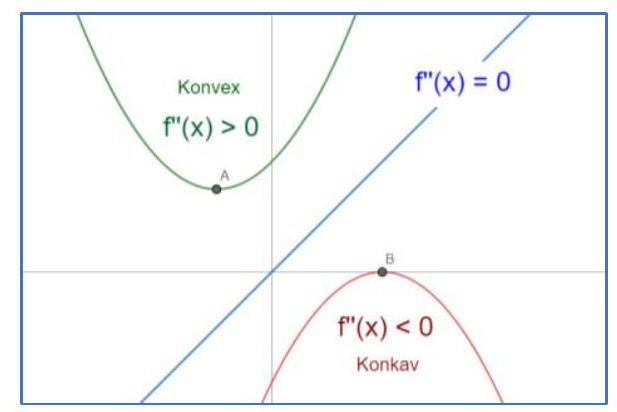
\includegraphics[scale=0.2]{Analysis1/zsf/Images/Integral/2024_01_20_7bfda6c084929ccc01ffg-07.jpg}
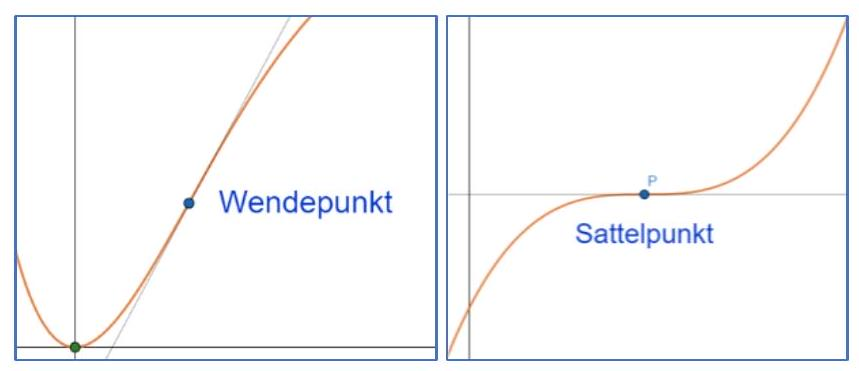
\includegraphics[scale=0.15]{Analysis1/zsf/sections/diff_funktionen/2024_01_20_7bfda6c084929ccc01ffg-08.jpg}
\begin{definition}{Wende- und Sattelpunkte}
    Als Wendepunkte werden Punkte bezeichnet bei denen sich der «Drehsinn» ändert. Wendepunkte mit horizontaler Tangente werden als Sattelpunkte oder Terrassenpunkte bezeichnet\\

Wendetangente:
\begin{itemize}
  \item Tangente an einem Wendepunkt
\end{itemize}
\end{definition}



\begin{KR}{Berechnung Wendetangente}
    Ermittlung durch Lösen der Gleichung $f^{\prime \prime}(x)=0 \rightarrow x_{0}$.\\
    Bedingungen:\\
    Sei $y=f(x)$ dreimal differenzierbar

\begin{itemize}
  \item $f^{\prime \prime}\left(x_{0}\right)=0$
  \item $f^{(3)}\left(x_{0}\right) \neq 0 \quad \rightarrow$ Wendepunkt
  \item Falls zusätzlich $f^{\prime}\left(x_{0}\right)=0 \quad \rightarrow$ Sattelpunkt
\end{itemize}
    
\end{KR}

\begin{concept}{Allgemeines Kriterium}\\
    Sei $f(x)$ eine genügend oft differenzierbare Funktion

\begin{itemize}
  \item $f^{\prime}\left(x_{0}\right)=0$
\end{itemize}

Sei $n$ die Ordnung der ersten nicht verschwindenden Ableitung von $f(x)$ an der Stelle $x_{0}$:

\begin{itemize}
  \item $f^{\prime}\left(x_{0}\right)=f^{\prime \prime}\left(x_{0}\right)=\cdots=f^{(n-1)}\left(x_{0}\right)=0$
  \item $f^{(n)}\left(x_{0}\right) \neq 0$
\end{itemize}

Schlussfolgerungen:
\begin{itemize}
    \item Wenn $n$ gerade, dann gibt es ein relatives Extremum $\left(f^{(n)}\left(x_{0}\right) \neq 0\right)$
    \item Wenn $n$ ungerade, dann hat $f(x)$ an der Stelle $x_{0}$ einen Wendepunkt und damit einen Sattelpunkt
\end{itemize}
\end{concept}

\begin{KR}{Vorgehen Wende- und Sattelpunkte}
    \begin{enumerate}
  \item Erste und zweite Ableitung

  \item Wendepunkt bestimmen

\end{enumerate}

\begin{itemize}
  \item $f^{\prime \prime}\left(x_{0}\right)=0 \rightarrow x_{0}$
  \item $f^{(3)}\left(x_{0}\right) \neq 0$
\end{itemize}

\begin{enumerate}
  \setcounter{enumi}{2}
  \item Sattelpunkte bestimmen
\end{enumerate}

\begin{itemize}
  \item $f^{\prime}\left(x_{0}\right)=0$
  \item $f^{\prime \prime}\left(x_{0}\right)=0$
  \item ...
  \item $f^{(n)}\left(x_{0}\right) \neq 0$
  \item Gerade $\rightarrow$ relatives Extremum
  \item Ungerade $\rightarrow$ Sattelpunkt
\end{itemize}

\begin{enumerate}
  \setcounter{enumi}{3}
  \item $x_{0}$ in ursprüngliche Gleichung einsetzen
\end{enumerate}
\end{KR}












                            \begin{definition}{Relative Extrema}
    \begin{itemize}
      \item Relative Extremal-Stelle $x_0$ $\quad \Longrightarrow \quad$ Minimal-/Maximalstelle
    
      \item Relatives Extremum $y_0$ $\quad \Longrightarrow \quad$ Maximum/Minimum
    
      \item Relativer Extremal-Punkt $P_0 = (x_0, y_0)$ $\quad \Longrightarrow \quad$ Hoch-/Tiefpunkt
    
    \end{itemize}
\end{definition}

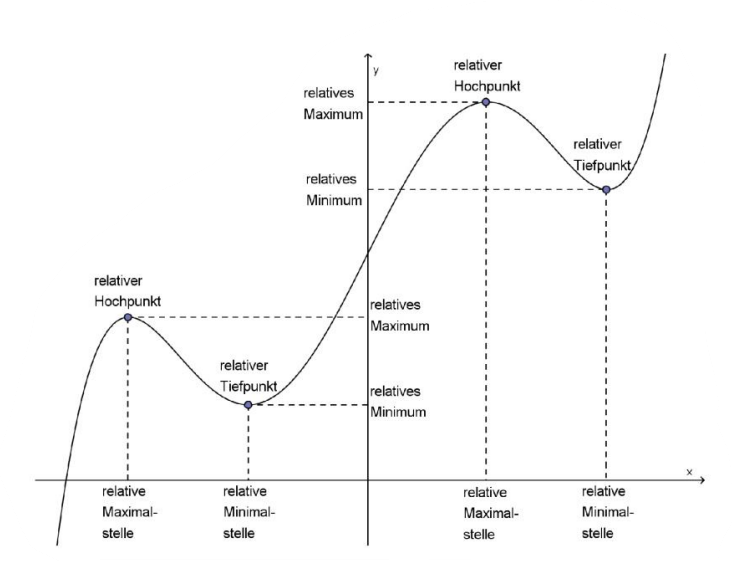
\includegraphics[scale=0.45]{Analysis1/zsf/Images/Differential/relative maxima.png}

\begin{KR}{Vorgehen relative Extrema} von $f(x) = y$:
    \begin{enumerate}
	\item Bestimme $f'(x)$ (Erste Ableitung)
	\item Bestimme NST von $f'(x)$\\
		$f'(x) = 0$ $ \Rightarrow$ $x$ lokales Extremum
	\item Bestimme $f''(x)$ (Zweite Ableitung)
		\begin{itemize}
			\item $f''(x) = 0$ $ \Rightarrow$ siehe Vorgehen Wende- und Sattelpunkte
			\item $f''(x) < 0$ $ \Rightarrow$ relatives Maximum
			\item $f''(x) > 0$ $ \Rightarrow$ relatives Minimum
		\end{itemize}
    \item In Gleichung f(x) = y einsetzen
        \begin{itemize}
            \item Hochpunkt/Tiefpunkt = $P(x, y)$
        \end{itemize}
\end{enumerate}
\end{KR}

\begin{example}
    $$
    \text{Beispiel: }f(x)=x^{5}-\frac{65}{3} x^{3}+180 x
    $$
    
    \begin{enumerate}
        \item $y^{\prime}=5 x^{4}-65 x^{2}+180$
    
        \item $y^{\prime}=0$
            \begin{itemize}
                \item $\rightarrow x_{0}=2 \pm \sqrt{3}$
            \end{itemize}
        \item $y^{\prime \prime}=20 x^{3}-130 x$
    
        \item $f^{\prime \prime}\left(x_{0}\right)=20 \cdot(2 \pm \sqrt{3})^{3}-130 \cdot(2 \pm \sqrt{3})$
            \begin{itemize}
              \item $f^{\prime \prime}(2-\sqrt{3})=-34 \rightarrow$ Maximum
              \item $f^{\prime \prime}(2+\sqrt{3})=554 \rightarrow$ Minimum
            \end{itemize}
        \item Gleichung $f\left(x_{0}\right)=y_{0}$
            \begin{itemize}
                \item Hochpunkt $/$ Tiefpunkt $=P\left(x_{0}, y_{0}\right)$
            \end{itemize}
    \end{enumerate}
\end{example}






                            \begin{formula}{Quadratische Funktionen}
$$y=a x^{2}+b x+c$$

    Nullstellen
    
    \begin{itemize}
      \item $y=a\left(x-x_{1}\right)\left(x-x_{2}\right)$
      \item $x_{0}=\frac{-b \pm \sqrt{b^{2}-4 a c}}{2 a}$
    \end{itemize}
    
    Scheitelpunkt
    
    \begin{itemize}
      \item $y=a\left(x-x_{0}\right)^{2}+y_{0}$
      \item $\mathrm{S}=\left(-\frac{b}{2 a}, \frac{4 a c-b^{2}}{4 a}\right)$
    \end{itemize}
\end{formula}
                           
                            
                            \raggedcolumns
                            \columnbreak
                            s\\
                            \raggedcolumns
                            \columnbreak
                            

                \section{Integralrechnung}
                            
\begin{theorem}{Fundamentalsatz}
	Seien $a<b$ und $f:[a,b] \to \R$ stetig.
	Die Funktion $F(x) = \int_{a}^{x} f(t) \dif t \quad a \leq x \leq b$ ist in $[a,b]$ stetig differenzierbar und $F'(x) f(x) \quad \forall x \in [a,b]$.
\end{theorem}
\begin{definition}{Stammfunktion}
	Seien $a<b$ und $f:[a,b] \to \R$ stetig.
	Eine Funktion $F. [a,b] \to \R$ heisst \emph{Stammfunktion} von $f$, falls $F$ (stetig) differenzierbar in $[a,b]$ ist und $F' = f$ in $[a,b]$ gilt.\\
    Die Stammfunktion $F$ von $f$ ist bis auf eine additive Konstante eindeutig bestimmt und es gilt:
    $\int_{a}^{b} f(x) \dif x = F(b) - F(a)$
\end{definition}











                            
                        
                            \subsubsection{Unbestimmte Integrale}
                                
\begin{definition}{Unbestimmtes Integral}
    Sei $f: I \to \R$ auf einem Intervall $I \subseteq \R$ definiert.
    Falls $f$ stetig ist, gibt es eine Stammfunktion $F$ für $f$.\\
    $\int f(x) \dif x = F(x) + C$\\
    Das unbestimmte Integral ist die Umkehroperation zur Ableitung.
\end{definition}

\begin{concept}{Integralregeln}
    \begin{itemize}
      \item Addition/Subtraktion
      $$\int f(x-k) d x=F(x-k)+C$$
      \item Multiplikation
      $$\int f(x \cdot k) d x=\frac{1}{k} F(x \cdot k)+C$$
      \item Skalarmultiplikation
      $$\int \lambda_{1} f(x)+\lambda_{2} g(x) d x=\lambda_{1} F(x)+\lambda_{2} G(x)+C$$
    \end{itemize}
\end{concept}   


                                

                            \subsubsection{Bestimmte Integrale}
                                \begin{definition}{Bestimmtes Integral}
    Für ein bestimmtes Integral von $f$ über $[a, b]$ schreibt man:

    $$\int_{a}^{b} f(x) d x$$
    
    Sei $f(x)$ eine im Intervall $[a, b]$ stetige Funktion:
    
    $$F^{\prime}{ }_{a}(x)=\frac{d}{d x}\left(\int_{a}^{x} f(t) d t\right)=f(x)$$

    Sei $f(x)$ eine im Intervall $[a, b]$ stetig Funktion, und sei $F(x)$ eine beliebige Stammfunktion von $f(x)$:

    $$\int_{a}^{b} f(t) d t=F(b)-F(a)$$
\end{definition}

\begin{concept}{Rechnen mit bestimmten Integralen}\\
	    Seien $a < b < c$ und $f: [a,b] \to \R$ beschränkt mit $f|_{[a,b]}$ und $f|_{[b,c]}$ integrierbar, sowie $\lambda_1, \lambda_2 \in \R$. Dann gilt:
    \begin{equation*}
    	\int_a^c f(x) \dif x = \int_a^b f(x) \dif x + \int_b^c f(x) \dif x
    \end{equation*}
    und erweitert (mit Skalaren):
    \begin{equation*}
    		\int_a^b \left( \lambda_1 f_1 (x) + \lambda_2 f_2 (x) \right) \dif x = \lambda_1 \int_a^b f_1(x) \dif x + \lambda_2 \int_a^b f_2(x) \dif x
    \end{equation*}
\end{concept}
                                \raggedcolumns
                                \columnbreak
                                \subsection{Integrale Berechnen}
                                
\begin{KR}{Strategie}
    \\\emph{Bruchform:}
    \begin{enumerate}
        \item Vereinfache, so dass ein einfacher Nenner entsteht
        \item Partialbruchzerlegung
        \item $\frac{u'}{2\sqrt{u}}$ oder $\frac{u'}{u}$ erkennen $\Rightarrow \sqrt{u}$ oder $log|u|$
    \end{enumerate}
    \emph{Produktform:}
    \begin{enumerate}
        \item Partielle Integration anwenden (evtl. mehrmals)
        \item Kettenregel verwenden
    \end{enumerate}
    \emph{Potenzen:}\\
        $\int_{a}^{b} f(x)^{c} d x$ umformen in $\int_{a}^{b}\left(f(x)^{c} \cdot 1\right) d x$ oder $\int_{a}^{b}\left(f(x)^{c-1} \cdot f(x)\right) d x$ um dann partielle Integration anzuwenden\\
    \emph{Exponentenform:}\\
        $e / \log$ Trick verwenden, wenn Variabel im Exponenten ist.\\
    \emph{Produkt mit $e, \sin , \cos$}\\
        Mehrmals partielle Integration anwenden, wobei sin, cos immer $g^{\prime}$ und immer $f$ ist.\\
    \emph{Summe im Integral:}\\
        Summe aus dem Integral herausziehen (dafür muss die Reihe gleichmässig konvergieren)
\end{KR}

                                


\begin{KR}{Flächeninhalt bei wechselndem Vorzeichen von $f(x)$}\\
\begin{itemize}
  \item $[a, b]=$ Intervall
  \item $x_{1}, x_{2}, \ldots, x_{n}=$ Nullstellen
\end{itemize}

$$\left|\int_{a}^{x_{1}} f(x) d x\right|+\left|\int_{x_{1}}^{x_{2}} f(x) d x\right|+\cdots+\left|\int_{x_{n}}^{b} f(x) d x\right|$$
\end{KR}

\begin{center}
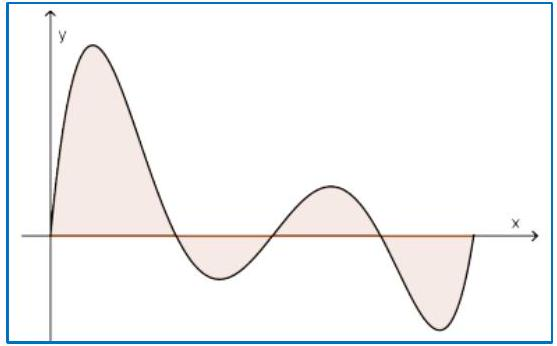
\includegraphics[scale=0.25]{Analysis1/zsf/Images/Integral/2024_01_20_7bfda6c084929ccc01ffg-06(1).jpg}
\end{center}

\begin{KR}{Flächeninhalt zwischen zwei Kurven $f(x)$ und $g(x)$}\\
\begin{itemize}
  \item $[a, b]=$ Intervall
  \item $x_{1}, x_{2}, \ldots, x_{n}=$ Schnittpunkte
\end{itemize}
$$\left|\int_{a}^{x_{1}}(f(x)-g(x)) d x\right|+\left|\int_{x_{1}}^{x_{2}}(f(x)-g(x))\right|+\cdots+\left|\int_{x_{n}}^{b}(f(x)-g(x))\right|$$
\end{KR}

\begin{center}
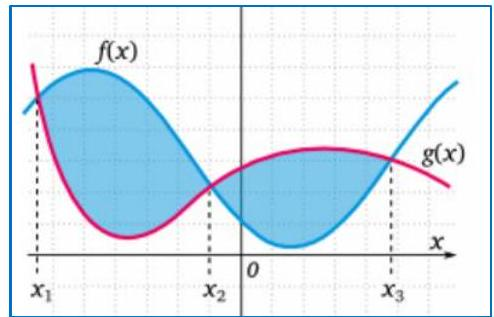
\includegraphics[scale=0.25]{Analysis1/zsf/Images/Integral/2024_01_20_7bfda6c084929ccc01ffg-06(2).jpg}
\end{center}


                                \raggedcolumns
                                \columnbreak
                                

\begin{highlight}{Wichtige Stammfunktionen}
        $\int f(x) \Longrightarrow F(x) + C$
    \begin{center}
        \begin{minipage}{0.45\linewidth}
            \tcbsubtitle{Potenzfunktionen}
            \begin{align*}
                &\int x^n \dif x  &=&  \quad \frac{1}{n+1}x^{n+1}  \\
                &\int \frac{f'}{f} \dif x  &=&  \quad \ln \left\lvert f \right\rvert  \\
                &\int \frac{1}{x} \dif x  &=& \quad \ln \left\lvert x \right\rvert  \\
                &\int \frac{1}{x+a} \dif x  &=&  \quad \ln \left\lvert x+a \right\rvert \\
                &\int \frac{1}{(x+a)^2} \dif x  &=&  -\frac{1}{x+a}  \\
                &\int \frac{1}{\sqrt{x}}\dif x  &=&  2 \sqrt{x}  \\
            \end{align*}
        \end{minipage}
        \hfill\vline\hfill
        \begin{minipage}{0.45\linewidth}
            \tcbsubtitle{Exponential- und Logarithmusfunktionen}
            \begin{align*}
                &\int\left(e^{x}\right) d x  &=& e^{x} \\
                &\int e^{ax} \dif x  &=&  \frac{1}{a} e^{ax}  \\
                &\int\left(a^{x}\right) d x \quad  &=& \frac{a^{x}}{\ln (\mathrm{a})} \\
                &\int(\ln (x)) d x  &=& x \cdot \ln (x)-x \\
                &\int\left(\log _{a}(x)\right) d x  &=& \frac{x \cdot \ln (x)-x}{\ln (\mathrm{a})} \\
            \end{align*}
        \end{minipage}
    \end{center}
    \tcbsubtitle{Geometrische Funktionen}
    \begin{center}
        \begin{minipage}{0.4\linewidth}
                \begin{align*}
                    &\int\cos (x) d x  &=& \sin (x) \\
                    &\int\sin (x) d x  &=& -\cos (x) \\
                    &\int\tan (x) d x  &=& -\ln |\cos (x)| \\
                    &\int \sin(ax)\dif x  &=&  - \frac{1}{a} \cos(a x)  \\
                    &\int \sin^2(ax)\dif x  &=&  \frac{x}{2} - \frac{1}{4a} \sin(2 a x)  \\
        			&\int \cos(ax)\dif x  &=&  \frac{1}{a} \sin(a x)  \\
        			&\int \cos^2(ax)\dif x  &=&  \frac{x}{2} + \frac{1}{4a} \sin(2 a x)  \\
                \end{align*}
        \end{minipage}
        \hfill\vline\hfill
        \begin{minipage}{0.45\linewidth}
            \begin{align*}
                    &\int\frac{1}{1+\mathrm{x}^{2}} d x  &=& \arctan (\mathrm{x})\\
                    &\int\frac{1}{\sqrt{1-x^{2}}} d x  &=& \arcsin (x) \\
                    &\int -\frac{1}{\sqrt{1-x^{2}}} d x  &=& \arccos (x) \\
        			&\int \frac{1}{\sqrt{1-x^2}}\dif x  &=&  \arcsin(x)  \\
        			&\int -\frac{1}{\sqrt{1-x^2}}\dif x  &=&  \arccos(x)  \\
        			&\int \frac{1}{1+x^2}\dif x  &=&  \arctan(x)  \\
            \end{align*}
        \end{minipage}
    \end{center}
\end{highlight}



                                \begin{KR}{Trick Gerade/Ungerade}
    Für ungerade Funktionen gilt $\int_{-a}^{+a} f(x) \dif x = 0$.
    \begin{itemize}
        \item Summe/Komposition: ungerade und ungerade
        \item Produkt/Quotient: ungerade und gerade
        \item Ableitung: gerade $\longrightarrow$ ungerade
    \end{itemize}
    Bsp ungerade: $f(x)$ = $-x$, $x$, $sin(x)$, $tan(x)$, Polynomfunktionen mit ungeradem Exponent\\
    gerade: $1$, $x^2$, $cos(x)$, $sec(x)$, Polynomf. mit geradem Exponent\\
    beides: $f(x) = 0$
\end{KR}

\begin{example}
	Berechne $\int_{-\infty}^{+\infty} \sin(x)\exp\left(-x^2\right) \dif x$\\ \\
	Wir wissen für die Funktionen:\\
        $\sin(x)$ $\to$ ungerade und $\exp(-x^2)$ $\to$ gerade\\ 
	Das Produkt einer ungeraden und geraden Funktion ist eine ungerade Funktion.\\
	Für ungerade Funktionen gilt $\int_{-a}^{+a} f(x) \dif x = 0$. Daraus folgt: 
	$\int_{-\infty}^{+\infty} \sin(x)\exp\left(-x^2\right) \dif x = 0$
\end{example}
                                
                                \raggedcolumns
                                \columnbreak
                                
                            \subsection{Komplexere Verfahren}
                            \subsubsection{Partielle Integration}
                                \begin{example}
    Berechne $\int_a^b \ln^2(t) \dif t$ mit partieller Integration.\\
    1. Mal Part.Int.: $g'(t) = 1 \rightarrow g(t) = t$ und $
            f(t) = \ln^2 (t) \rightarrow  f'(x) = \frac{2 \cdot \ln(t)}{t}$
    \begin{gather*}
        \int_a^b \ln^2(t) \dif t = \left[t \cdot \ln^2(t)\right]_a^b - \int_a^b t \cdot \frac{2 \cdot \ln(t)}{t} \dif t = {\color{blue}(*)}
    \end{gather*}
    2. Mal Part.Int.: $g'(t) = 1 \rightarrow g(t) = t$ und $
            f(t) = \ln (t) \rightarrow f'(x) = \frac{1}{t}$
    \begin{gather*}
        {\color{blue}(*)} = \left[t \cdot \ln^2(t)\right]_a^b - 2 \left(\left[t \cdot \ln (t)\right]_a^b - \int_a^b 1 \dif t\right)
    \end{gather*}
\end{example}

                                \begin{example}
    Berechne $\int_a^b \ln^2(t) \dif t$ mit partieller Integration.\\
    1. Mal Part.Int.: $g'(t) = 1 \rightarrow g(t) = t$ und $
            f(t) = \ln^2 (t) \rightarrow  f'(x) = \frac{2 \cdot \ln(t)}{t}$
    \begin{gather*}
        \int_a^b \ln^2(t) \dif t = \left[t \cdot \ln^2(t)\right]_a^b - \int_a^b t \cdot \frac{2 \cdot \ln(t)}{t} \dif t = {\color{blue}(*)}
    \end{gather*}
    2. Mal Part.Int.: $g'(t) = 1 \rightarrow g(t) = t$ und $
            f(t) = \ln (t) \rightarrow f'(x) = \frac{1}{t}$
    \begin{gather*}
        {\color{blue}(*)} = \left[t \cdot \ln^2(t)\right]_a^b - 2 \left(\left[t \cdot \ln (t)\right]_a^b - \int_a^b 1 \dif t\right)
    \end{gather*}
\end{example}

                            
                            
                               
                    
                            \subsubsection{Partialbruchzerlegung}
                                \begin{example}
	Berechne $\int \frac{x+1}{x^3 + x^2 - 6x} \dif x$ mittels PBZ.
	\begin{gather*}
		\frac{x+1}{x^3 + x^2 - 6x} = \frac{x+1}{x(x-2)(x+3)} = \frac{A}{x} + \frac{B}{x-2} + \frac{C}{x+3}\\
		\Rightarrow A + B + C = 0 \quad A + 3B - 2C = 1 \quad -6A = 1
	\end{gather*}
	Daraus folgt: $A = -\frac{1}{6}$, $B = \frac{3}{10}$, $C = -\frac{2}{15}$
	\begin{align*}
		\int \frac{x+1}{x^3 + x^2 - 6x} \dif x &= -\frac{1}{6} \int \frac{1}{x} \dif x + \frac{3}{10} \int \frac{1}{x-2} \dif x - \frac{2}{15} \int \frac{1}{x+3} \dif x\\
						       &= -\frac{1}{6} \log |x| + \frac{3}{10} \log |x-2| - \frac{2}{5} \log |x+3| + C 
	\end{align*}
\end{example}
                                \begin{example}
	Berechne $\int \frac{x+1}{x^3 + x^2 - 6x} \dif x$ mittels PBZ.
	\begin{gather*}
		\frac{x+1}{x^3 + x^2 - 6x} = \frac{x+1}{x(x-2)(x+3)} = \frac{A}{x} + \frac{B}{x-2} + \frac{C}{x+3}\\
		\Rightarrow A + B + C = 0 \quad A + 3B - 2C = 1 \quad -6A = 1
	\end{gather*}
	Daraus folgt: $A = -\frac{1}{6}$, $B = \frac{3}{10}$, $C = -\frac{2}{15}$
	\begin{align*}
		\int \frac{x+1}{x^3 + x^2 - 6x} \dif x &= -\frac{1}{6} \int \frac{1}{x} \dif x + \frac{3}{10} \int \frac{1}{x-2} \dif x - \frac{2}{15} \int \frac{1}{x+3} \dif x\\
						       &= -\frac{1}{6} \log |x| + \frac{3}{10} \log |x-2| - \frac{2}{5} \log |x+3| + C 
	\end{align*}
\end{example}
                                \begin{comment}
    Sei $R(x) = \frac{P(x)}{Q(x)}$ eine rationale Funktion. Dann lässt sich $\int R(x) \dif x$ als elementare Funktion darstellen.\\
Dh. als Funktion bestehend aus Polynomen, rationalen, exponentiellen, logarithmischen, trigonometrischen und/oder inversen trig. Funktionen.
Die Rechnung besteht aus 3 Schritten:
\begin{enumerate}
	\item Reduktion auf den Fall indem $\grad(P) < \grad(Q)$.
	\item Zerlegung von $Q$ in lineare und quadratische Faktoren, sowie Partialbruchzerlegung von $R$.
	\item Integration der Partialbrüche.
\end{enumerate}

\paragraph{Zu Schritt 1}
    Sei $R(x) = \frac{P(x)}{Q(x)}$. Falls $\grad(P) \geq \grad(Q)$ wenden wir den euklidischen Alg. an: $P(x) = S(x)Q(x) + \hat{P}(x)$, wobei $\grad \left( \hat{P} \right) < \grad{Q}$.
    Dann ist $\frac{P(x)}{Q(x)}  = S(x) + \frac{\hat{P}(x)}{Q(x)}$.
\paragraph{Zu Schritt 2}
	Seine $P,Q$ Polynome mit $\grad(P) < \grad(Q)$ und $Q$ mit Produktzerlegung $Q(x) = \prod_{j=1}^l \left( (x - \alpha_j)^2 + \beta_j^2 \right)^{m_j} \prod_{i=1}^k (x- \gamma_i)^{n_i}$.
    \\Dann gibt es $A_{ij}, B_{ij}, C_{ij}$ reelle Zahlen mit
\begin{equation*}
	\frac{P(x)}{Q(x)} = \sum^{l}_{i=1} \sum^{m_i}_{j=1} \frac{(A_{ij} + B_{ij}x)}{\left( (x-\alpha_i)^2 + \beta_i^2 \right)^j} + \sum^{k}_{i=1} \sum^{n_i}_{j=1} \frac{C_{ij}}{(x-\gamma_i)^j} 
\end{equation*}
\end{comment}

\begin{KR}{Stammfunktionen rationaler Funktionen}\\
    Die Stammfunktion einer Funktion $R(x)=\frac{P(x)}{Q(x)}$ bestehend aus rationalen Funktionen lässt sich als eine Funktion von Polynomen rationalen, exponentiallen, logarithmischen, trigonometrischen und inver trigonometrischen Funktionen darstellen.

Zuerst wollen wir das $\operatorname{grad}(P)<\operatorname{grad}(Q)$ gilt, falls die nicht der Fall ist uhren wir Polynomdivision aus. Danach bestimmen wir alle reellen und komenter Nun gilt:

$$
R(x)=\sum_{k=1}^{N} R_{k}(x)+\sum_{k=1}^{M} Z_{k}(x)
$$

Hier ist $N$ die Anzahl reeller Nullstellen und $M$ die Anzahl der komplexen Nullstellen. Es gilt:

$$
\begin{gathered}
R_{k}(x)=\frac{a_{k_{1}}}{\left(x-x_{k}\right)}+\frac{a_{k_{2}}}{\left(x-x_{k}\right)^{2}}+\ldots+\frac{a_{k_{n_{k}}}}{\left(x-x_{k}\right)^{n_{k}}} \\
Q_{k}(x)=\frac{a_{k_{1}}+b_{k_{1}} x}{\left(\left(x-\alpha_{k}\right)^{2}+\beta_{k}^{2}\right)}+\ldots+\frac{a_{k_{m_{k}}}+b_{k_{m_{k}}} x}{\left(\left(x-\alpha_{k}\right)^{2}+\beta_{k}^{2}\right)^{m_{k}}}
\end{gathered}
$$

Somit können wir die Funktion mit Partialbruchzerlegung in einzelnen Brüchen darstellen, welche dann leichter zu integrieren sind. Wenn wi eine reelle Nullstelle haben so gil:

$$
\int \frac{1}{\left(x-\gamma_{i}\right)^{n}}=\left\{\begin{array}{l}
\ln \left(x-\gamma_{i}\right) \quad \text { für } n=1 \\
\frac{-1}{(n-1)\left(x \gamma_{i}\right)^{n-1}}
\end{array}\right.
$$

Für komplexe Nullstellen gilt:

$$
\begin{gathered}
\frac{A+B x}{\left((x-\alpha)^{2}+\beta^{2}\right)^{j}}=\frac{B(x-\alpha)}{\left((x-\alpha)^{2}+\beta^{2}\right)^{j}}+\frac{A+B \alpha}{\left((x-\alpha)^{2}+\beta^{2}\right)^{j}} \\
\int \frac{B(x-\alpha)}{\left((x-\alpha)^{2}+\beta^{2}\right)^{j}}=\left\{\begin{array}{l}
\frac{B}{2} \ln \left((x-\alpha)^{2}+\beta^{2}\right)^{j} \quad \text { für } j=1 \\
\frac{B}{(2(1-j))\left((x-\alpha)^{2}+\beta^{2}\right)^{j-1}}
\end{array}\right.
\end{gathered}
$$

Für den letzen Term brauchen wir die Substitution $(x-\alpha)=\beta t$

$$
\int \frac{A+B \alpha}{\left((x-\alpha)^{2}+\beta^{2}\right)^{j}}=\frac{A+B \alpha}{\beta^{2 j-1}} \cdot \int \frac{1}{\left(t^{2}+1\right)^{j}} d t
$$
\end{KR}

\begin{example}
    Bsp.

$$
\int \frac{x^{2}-x+2}{x^{3}-x^{2}+x-1}
$$

Wir finden die erste Nullstelle $(x-1)$ durch ausprobieren. Danach führen wir Polynomdivision (durch $x-1$ ) aus und erhalten damit die weite Nullstelle $\left(x^{2}+1\right)$, Da $x^{2}+1$ eine komplexe Nullstelle ist, nehme wir dafür $A+B x$

$$
\frac{A+B x}{x^{2}+1}+\frac{C}{x-1}=\frac{x^{2}-x+2}{\left(x^{2}+1\right)(x-1)}
$$

$\Longrightarrow x^{2}-x+2=(A+C) \cdot x^{2}+(B-A) x+(C-B) \cdot 1$

$\Longrightarrow B=0, A=-1, C=1$

$\Longrightarrow \int \frac{1}{x-1}+\frac{-1}{x^{2}+1}=\ln (x-1)-\arctan (x)+C$
\end{example}




                                \subsubsection{Substitution}
                                
\begin{concept}{Substitution}\\
    Die Substitution ist die Umkehrung der Kettenregel. D.h. wir wollen Substitution vorallem verwenden, wenn wir innere Funktionen haben.
    \begin{equation*}
        \int_{g(b)}^{g(a)} f(x) \dif x = \int_{a}^b f(g(t)) g'(t) \dif t
    \end{equation*}
    bzw. für unbestimmte Integrale

    $$
    \int f(g(t)) \cdot g^{\prime}(t) d t=\left.\int f(x) d x\right|_{x=g(t)}
    $$
\end{concept}



\begin{formula}{Nützliche Substitutionen}
    \begin{itemize}
        \item $e^{x}, \sinh (x), \cosh (x)$, subst: $t=e^{a x}, d x=\frac{d t}{a t}$ Dann $\sinh =\cosh =\frac{t^{2}-1}{2 t}$
        \item $\log (x)$ subst: $t=\log (x), x=e^{t}, d x=e^{t} d t$
        \item für gerade $n: \cos ^{n}(x), \sin ^{n}(x), \tan (x)$ Sub: $t=\tan (x)$, $d y=\frac{1}{1+t^{2}} d t, \sin ^{2}(x)=\frac{t^{2}}{1+t^{2}}, \cos ^{2}(x)=\frac{1}{1+t^{2}}$
        \item für ungerade $n: \cos ^{n}(x), \sin ^{n}(x)$, Sub: $t=\tan (x / 2)$, $d y=\frac{2}{1+t^{2}} d t, \sin (x)=\frac{2 t}{1+t^{2}}, \cos (x)=\frac{1-t^{2}}{1+t^{2}}$
        \item $\int \sqrt{1-x^{2}} d x$ sub: $x=\sin (x)$ oder $\cos (x)$
        \item $\int \sqrt{1+x^{2}} d x$ sub: $x=\sinh (x)$
    \end{itemize}
\end{formula}

\begin{example}
    Bsp. $\int \frac{x}{\sqrt{9-x^{2}}} d x$ substitution mit $t=\sqrt{9-x^{2}}$.

    $$
    \Rightarrow x=\sqrt{9-t^{2}} \Rightarrow x^{\prime}=\frac{-2 t}{2 \sqrt{9-t^{2}}} \Rightarrow d x=\frac{-t \cdot d t}{\sqrt{9-t^{2}}}
    $$
    
    $\int-d t=-t$ rücksubstitution $\Rightarrow-\sqrt{9-x^{2}}$
\end{example}

                            
\begin{concept}{Substitution}\\
    Die Substitution ist die Umkehrung der Kettenregel. D.h. wir wollen Substitution vorallem verwenden, wenn wir innere Funktionen haben.
    \begin{equation*}
        \int_{g(b)}^{g(a)} f(x) \dif x = \int_{a}^b f(g(t)) g'(t) \dif t
    \end{equation*}
    bzw. für unbestimmte Integrale

    $$
    \int f(g(t)) \cdot g^{\prime}(t) d t=\left.\int f(x) d x\right|_{x=g(t)}
    $$
\end{concept}



\begin{formula}{Nützliche Substitutionen}
    \begin{itemize}
        \item $e^{x}, \sinh (x), \cosh (x)$, subst: $t=e^{a x}, d x=\frac{d t}{a t}$ Dann $\sinh =\cosh =\frac{t^{2}-1}{2 t}$
        \item $\log (x)$ subst: $t=\log (x), x=e^{t}, d x=e^{t} d t$
        \item für gerade $n: \cos ^{n}(x), \sin ^{n}(x), \tan (x)$ Sub: $t=\tan (x)$, $d y=\frac{1}{1+t^{2}} d t, \sin ^{2}(x)=\frac{t^{2}}{1+t^{2}}, \cos ^{2}(x)=\frac{1}{1+t^{2}}$
        \item für ungerade $n: \cos ^{n}(x), \sin ^{n}(x)$, Sub: $t=\tan (x / 2)$, $d y=\frac{2}{1+t^{2}} d t, \sin (x)=\frac{2 t}{1+t^{2}}, \cos (x)=\frac{1-t^{2}}{1+t^{2}}$
        \item $\int \sqrt{1-x^{2}} d x$ sub: $x=\sin (x)$ oder $\cos (x)$
        \item $\int \sqrt{1+x^{2}} d x$ sub: $x=\sinh (x)$
    \end{itemize}
\end{formula}

\begin{example}
    Bsp. $\int \frac{x}{\sqrt{9-x^{2}}} d x$ substitution mit $t=\sqrt{9-x^{2}}$.

    $$
    \Rightarrow x=\sqrt{9-t^{2}} \Rightarrow x^{\prime}=\frac{-2 t}{2 \sqrt{9-t^{2}}} \Rightarrow d x=\frac{-t \cdot d t}{\sqrt{9-t^{2}}}
    $$
    
    $\int-d t=-t$ rücksubstitution $\Rightarrow-\sqrt{9-x^{2}}$
\end{example}

                                \begin{example}
    Berechne $\int_0^{\pi/2} \frac{e^{-\tan (x)}}{cos^2(x)} \dif x$. Finde Stammfunktion, indem man bemerkt:
    \begin{equation*}
        \left(e^{\tan(x)}\right)' \underset{4.11}{\overset{\text{Ket.R}}{=}} e^{\tan(x)} \frac{1}{\cos^2(x)} \Longrightarrow \left(-e^{-\tan(x)}\right)' = \frac{e^{-\tan(x)}}{\cos^2(x)}
    \end{equation*}
    
    \begin{equation*}
       \text{und dementsprechend:} \int_0^{\frac{\pi}{2}} \frac{e^{-\tan (x)}}{\cos^2(x)} \dif x = \left[-e^{-\tan(x)}\right]_0^{\frac{\pi}{2}}
    \end{equation*}
\end{example}

                            \raggedcolumns
                            \columnbreak

                            \begin{KR}{Integrieren von Flächen}
Nullstellen bestimmen: $=>$ Fläche oberhalb $\mathrm{x}$ Achse, + Fläche evtl unterhalb x Achse...
\end{KR}

\begin{KR}{Transformation: Funktionen zeichnen}
    \begin{itemize}
    \item $y=f(x) B y=f(a x)$ : Streckung des Graphen um Faktor $\frac{1}{a}$ in x Richtung
  \item $y=f(x)$ ß $y=f(x+b)$ : Verschiebung des Graphen um $|b|$ in $\mathbf{x}$ Richtung
  \item $y=f(x)$ ß $y=c f(x)$ : Streckung des Graphen um Faktor $c$ in y Richtung
  \item $y=f(x)$ ß $y=f(x)+d$ : Verschiebung des Graphen um $d$ Einheiten in y Richtung
\end{itemize}
\end{KR}

\begin{concept}{Graphen von Polynomen}
    \begin{itemize}
  \item Hat so viele Nullstellen wie Grad des Polynoms (Fundamentalssatz der Algebra)
  \item bei Faktorisiertem angeben, noch Vorfaktor beachten $=>$ Falls Punkt gegeben kann dieser berechnet werden
  \item für jede Nullstelle:
  \item Einfach: Schneidend
  \item Doppelt: Berührend
  \item Dreifach: Wie $x^{3}$
  \item für Asymptoten: anlehnend
\end{itemize}
\end{concept}

\includegraphics[scale=0.4]{Analysis1/pics/2024_01_22_0c4ec55175f5e3a7f87dg-2(1).jpg}

\begin{concept}{Horner-Schema}
    Um nach Nullstellen aufzulösen: Nullstelle einsetzen und das Resultat (ohne Null am Ende) mit Grad -1 auffüllen = Lösung der Polynom Division...\\
    Im Beispiel: Rest würde als $+0 /$ ( $x-5$ ) angefügt werden
\end{concept}

\includegraphics[scale=0.3]{Analysis1/pics/2024_01_22_0c4ec55175f5e3a7f87dg-2(2).jpg}

\begin{KR}{Monotonie zeigen}
    \begin{itemize}
  \item $a_{n+1}-a_{n} \geq 0 \Rightarrow$ monoton wachsend (bzw. umgekehrt fallend)
  \item $\frac{a_{n+1}}{a_{n}} \geq 1$ und $a_{n} \geq 0$ dann monoton wachsend
\end{itemize}
\end{KR}

\begin{KR}{Grenzwert Berechnen Tricks}
\begin{itemize}
  \item " $\frac{\infty}{\infty} "$ Trick: Erweitern mit $\frac{1}{n^{k}}$ (k: grösster Exponent)
\end{itemize}

$\lim _{n \rightarrow \infty} \frac{2 n^{6}-n^{3}}{7 n^{6}+n^{5}-3} \cdot \frac{\frac{1}{n^{6}}}{\frac{1}{n^{6}}}=\frac{2}{7}$

\begin{itemize}
  \item " $\frac{\infty}{\infty} "$ Trick: Erweitern mit $\frac{1}{a^{k}}$ (a: grösste Basis, k: kleinster Exponent) $\lim _{n \rightarrow \infty} \frac{7^{n-1}+2^{n+1}}{7^{n}+5} \cdot \frac{\frac{1}{7^{n-1}}}{\frac{1}{7^{n-1}}}=\frac{1}{7}$
  \item " $\infty-\infty$ " Trick: Erweitern mit $\sqrt{\cdots}+\sqrt{\cdots}$
\end{itemize}

$\lim _{n \rightarrow \infty}\left(\sqrt{n^{2}+n}-\sqrt{n^{2}+1}\right)=1 / 2$

\begin{itemize}
  \item Kettenfunktionen: Trick Stetigkeit von $\mathrm{f}(\mathrm{x})$ ausnützen $\Rightarrow$ zuerst $\lim _{n \rightarrow \infty} a_{n}$ berechnen, danach $\mathrm{f}(\mathrm{x})$ (ohne nochmals lim) anwenden.
  \item e-like...: Trick: umformen zu $\left(\left(1+\frac{1}{x}\right)^{x}\right)^{a} \Rightarrow e^{a}$
\end{itemize}
\end{KR}

\begin{KR}{Kurvendiskussion}
    \begin{itemize}
  \item Monotonieverhalten (monoton wachsend / fallende Bereiche bestimmen)
  \item Krümmungsverhalten / Minima / Maxima etc überprüfen
  \item Kritische Punkte: hinreichende Bedingung nicht erfüllt
\end{itemize}

\begin{enumerate}
  \item Keine Aussage!

  \item Leite $\mathrm{f}(\mathrm{x})$ so lange ab bis die $n$-te Ableitung an Stelle $\neq 0$ ist. Dann gilt:

  \item Wenn $\mathrm{n}$ gerade ist, hat $\mathrm{f}(\mathrm{x})$ an der Stelle $\mathrm{x} 0$ ein relatives Extremum, und zwar ein relatives Maximum im Fall $f^{(n)}\left(x_{0}\right)<0$ und ein relatives Minimum im Fall $f^{(n)}\left(x_{0}\right)>0$

  \item Wenn $n$ ungerade ist, hat $f(x)$ an der Stelle $x_{0}$ einen Wendepunkt (und damit einen Sattelpunkt).

\end{enumerate}
\end{KR}

\begin{KR}{Differentialrechnung Tricks}
    \begin{itemize}
  \item Überall differenzierbar: Einheitliche Tangente (Ableitung 0 setzen) und dh: Grenzwerte müssen denselben Wert ergeben
  \item Zwei Funktionskurven berühren sich (aww): bedeutet dass sie an einer Stelle x0 den gleichen Funktionswert und die gleiche Ableitung haben
  \item Tangente bestimmen (Linearisierung): $f\left(x_{0}\right)+f^{\prime}\left(x_{0}\right)\left(x-x_{0}\right)$
\end{itemize}
\end{KR}

\begin{KR}{Extremwertaufgaben}
    \begin{enumerate}
  \item Gleichung aufstellen

  \item Ableiten

  \item Kandidaten für Min/Max finden

  \item Begründen durch 2. Ableitung / Graph

\end{enumerate}
\end{KR}

\begin{KR}{Ungleichungen}

No Flipping needed
    \begin{itemize}
  \item $\log _{a}()$ [mit a $>1$ 1] (oder andere monoton wachsende Funktion)
  \item Addition / Subtraktion
  \item Mult. mit Positiver Zahl
  \item Divi. durch Positive Zahl
\end{itemize}

Flipping needed

\begin{itemize}
  \item $\log _{a}()[$ mit $0<\mathrm{a}<1]$ (oder andere monoton fallende Funktion)
  \item Mult. mit Negativer Zahl
  \item Divi. durch Negative Zahl
\end{itemize}
\end{KR}

                                

                              
                              

                            

                            
                    
                
                
                 
            
                
               
                
                 
                
                
    
       

        
           
                
            

           
                

      
		
		
		
	\end{multicols*}
\end{document}
